%% template https://sdqweb.ipd.kit.edu/wiki/Dokumentvorlagen

\documentclass[en,16:9,smallfoot]{sdqbeamer}
\titleimage{banner_2020_kit}
\grouplogo{institute_blank}
\groupname{}%Institute AIFB}

\title[Data Mining and Information Extraction Methods for Large-Scale High Quality Representations of Scientific Publications]{Data Mining and Information Extraction Methods for Large-Scale\\High Quality Representations of Scientific Publications}
\subtitle{Dissertation Defense}
\author{Tarek Saier}

\date[22.\,04.\,2024]{22. April 2024}

% literature
\usepackage[citestyle=nature,bibstyle=nature,hyperref,backend=biber]{biblatex}
\addbibresource{presentation.bib}
\bibhang1em

% custom packages
% % heart symbol
\usepackage{graphicx,txfonts}
\newcommand{\heart}{\ensuremath\varheartsuit}
% % numeric references instead of paper symbols
\setbeamertemplate{bibliography item}{\insertbiblabel}
\renewcommand*{\bibfont}{\scriptsize}
% % backup slides
\usepackage{appendixnumberbeamer}
% % nice tables
\usepackage{threeparttable}
\usepackage{booktabs}
% % strike-through
\usepackage[normalem]{ulem}
% % % two monitor setup
% \usepackage{pgfpages}
% \setbeameroption{show notes on second screen}
\usepackage{subfig}
\usepackage{multirow}  % for multi row/col table cells
% colors
\usepackage{xcolor}

\definecolor{artifactblue}{HTML}{0059A0}
\definecolor{parametergreen}{HTML}{539A55}
\definecolor{valuered}{HTML}{CF8369}
\definecolor{contextgrey}{HTML}{A2A2A2}
% % infoboxes
\usepackage{fontawesome}
\usepackage[most]{tcolorbox}
\definecolor{pubgreen-box}{RGB}{112,214,167}
\definecolor{pubgreen-bg}{RGB}{247,247,244}
\definecolor{discussionpurp-box}{RGB}{181,145,180}
\definecolor{discussionpurp-bg}{RGB}{251,249,251}
\definecolor{lightgrey}{HTML}{CFCFCF}
\definecolor{infogrey-box}{RGB}{163,163,163}
\definecolor{infogrey-bg}{RGB}{250,250,250}
\definecolor{objblue-box}{RGB}{103,188,223}
\definecolor{objblue-bg}{RGB}{247,252,253}
\newtcolorbox{infobox-pub}{
    breakable,
    enhanced,
    arc=1pt,
    top=2pt,
    bottom=2pt,
    left=2pt,
    right=2pt,
    colback=pubgreen-bg,
    colframe=pubgreen-box,
    coltext=black,
    leftrule=24pt,
    overlay={%
     \begin{tcbclipframe}
      \node[anchor=center, xshift=12pt, yshift=-10pt, text=pubgreen-bg] at (frame.north west){\large\faFileText};
     \end{tcbclipframe}
    }
}
\newtcolorbox{infobox-pub-small}{
    breakable,
    enhanced,
    hbox,
    arc=1pt,
    top=2pt,
    bottom=2pt,
    left=2pt,
    right=2pt,
    colback=pubgreen-bg,
    colframe=pubgreen-box,
    coltext=black,
    leftrule=24pt,
    overlay={%
     \begin{tcbclipframe}
      \node[anchor=center, xshift=12pt, yshift=-10pt, text=pubgreen-bg] at (frame.north west){\large\faFileText};
     \end{tcbclipframe}
    }
}
\newtcolorbox{infobox-map}{
    breakable,
    enhanced,
    arc=1pt,
    top=5pt,
    bottom=5pt,
    left=2pt,
    right=2pt,
    colback=pubgreen-bg,
    colframe=kit-green100,
    coltext=black,
}
\newtcolorbox{infobox-discussion}{
    breakable,
    enhanced,
    arc=1pt,
    top=2pt,
    bottom=2pt,
    left=2pt,
    right=2pt,
    colback=discussionpurp-bg,
    colframe=discussionpurp-box,
    coltext=black,
    leftrule=24pt,
    overlay={%
     \begin{tcbclipframe}
      \node[anchor=center, xshift=12pt, yshift=-10pt, text=discussionpurp-bg] at (frame.north west){\large\faComments};
     \end{tcbclipframe}
    }
}
\newtcolorbox{infobox-info}{
    breakable,
    enhanced,
    arc=1pt,
    top=2pt,
    bottom=2pt,
    left=2pt,
    right=2pt,
    colback=infogrey-bg,
    colframe=infogrey-box,
    coltext=black,
    leftrule=24pt,
    overlay={%
     \begin{tcbclipframe}
      \node[anchor=center, xshift=12pt, yshift=-10pt, text=infogrey-bg] at (frame.north west){\large\faInfoCircle};
     \end{tcbclipframe}
    }
}
% \newtcolorbox{infobox-q}{
%     breakable,
%     enhanced,
%     arc=1pt,
%     top=2pt,
%     bottom=2pt,
%     left=2pt,
%     right=2pt,
%     colback=rqblue-bg,
%     colframe=rqblue-box,
%     coltext=black,
%     leftrule=24pt,
%     overlay={%
%      \begin{tcbclipframe}
%       \node[anchor=center, xshift=12pt, yshift=-10pt, text=rqblue-bg] at (frame.north west){\large\faQuestionCircle};
%      \end{tcbclipframe}
%     }
% }
\newtcolorbox{infobox-objective}{
    %breakable,
    enhanced,
    arc=1pt,
    colback=objblue-bg,
    colframe=objblue-box,
    coltext=black,
    leftrule=36pt,
    overlay={%
     \begin{tcbclipframe}
      \node[anchor=center, xshift=19pt, yshift=-18pt, text=objblue-bg] at (frame.north west){\Large\faCrosshairs};
     \end{tcbclipframe}
    }
}
% % /infoboxes
\newcommand{\rtmark}[1]{%
    \textbf{{\color{objblue-box}\faCrosshairs}\,RT#1}%
}
% \usepackage{enumitem}
% \newlist{rtlist}{enumerate}{1}
% \setlist[rtlist]{%
% labelindent=0em,%
% labelwidth=2cm,%
% labelsep*=0.5em,%
% leftmargin=!,%
% label=\rtmark{\arabic*}:,%
% }

\usepackage{makecell}
% Redefine the cellset for makecell to adjust the line height
\renewcommand\cellset{\renewcommand\arraystretch{0.8}\ignorespaces}

\begin{document}
% title slide
\KITtitleframe

% % toc
% \begin{frame}{toc}
% \tableofcontents
% \end{frame}

\section{Motivation}

   \begin{frame}[plain]
        \vspace{1cm}
        \centering
        \begin{Large}
        {\color{lightgrey}\textbf{Data Mining and Information Extraction Methods}}\\
        \vspace{0.25em}
        {\color{lightgrey}\textbf{for Large-Scale High Quality}}\\
        \vspace{0.5em}
        {\textbf{
            \only<1>{Representations of Scientific Publications}
            \only<2>{Scholarly Data}
        }}
        \end{Large}
   \end{frame}

   \begin{frame}{Scholarly Data}
   \begin{columns}
       \column{.575\textwidth}
        \begin{itemize}
            \item \textbf{Usage}
            \begin{itemize}
                \item Services {\color{contextgrey}(search, recommendation, statistics)}
                \item ML models {\color{contextgrey}(LLMs, sumarization, recommender systems)} % PILE, S2ORC, unarXive, ...)
                \item Analyses {\color{contextgrey}(temporal, geographic, institutional)}
            \end{itemize}
            \item \textbf{Flavors}
            \begin{itemize}
                \item Metadata {\color{contextgrey}(MAG, OpenAlex, ORKG, crossref)}
                \item Documents {\color{contextgrey}(Core, arXMLiv, PMC)}
                \item Linked Documents {\color{contextgrey}(unarXive, S2ORC)}
            \end{itemize}
            \item \textbf{Data Sources}
            \begin{itemize}
                \item PDF {\color{contextgrey}(Core, ACL Anthology)}
                \item XML {\color{contextgrey}(PubMed, PLOS, publisher internal)}
                \item LaTeX {\color{contextgrey}(arXiv)}
            \end{itemize}
        \end{itemize}
       \column{.375\textwidth}
            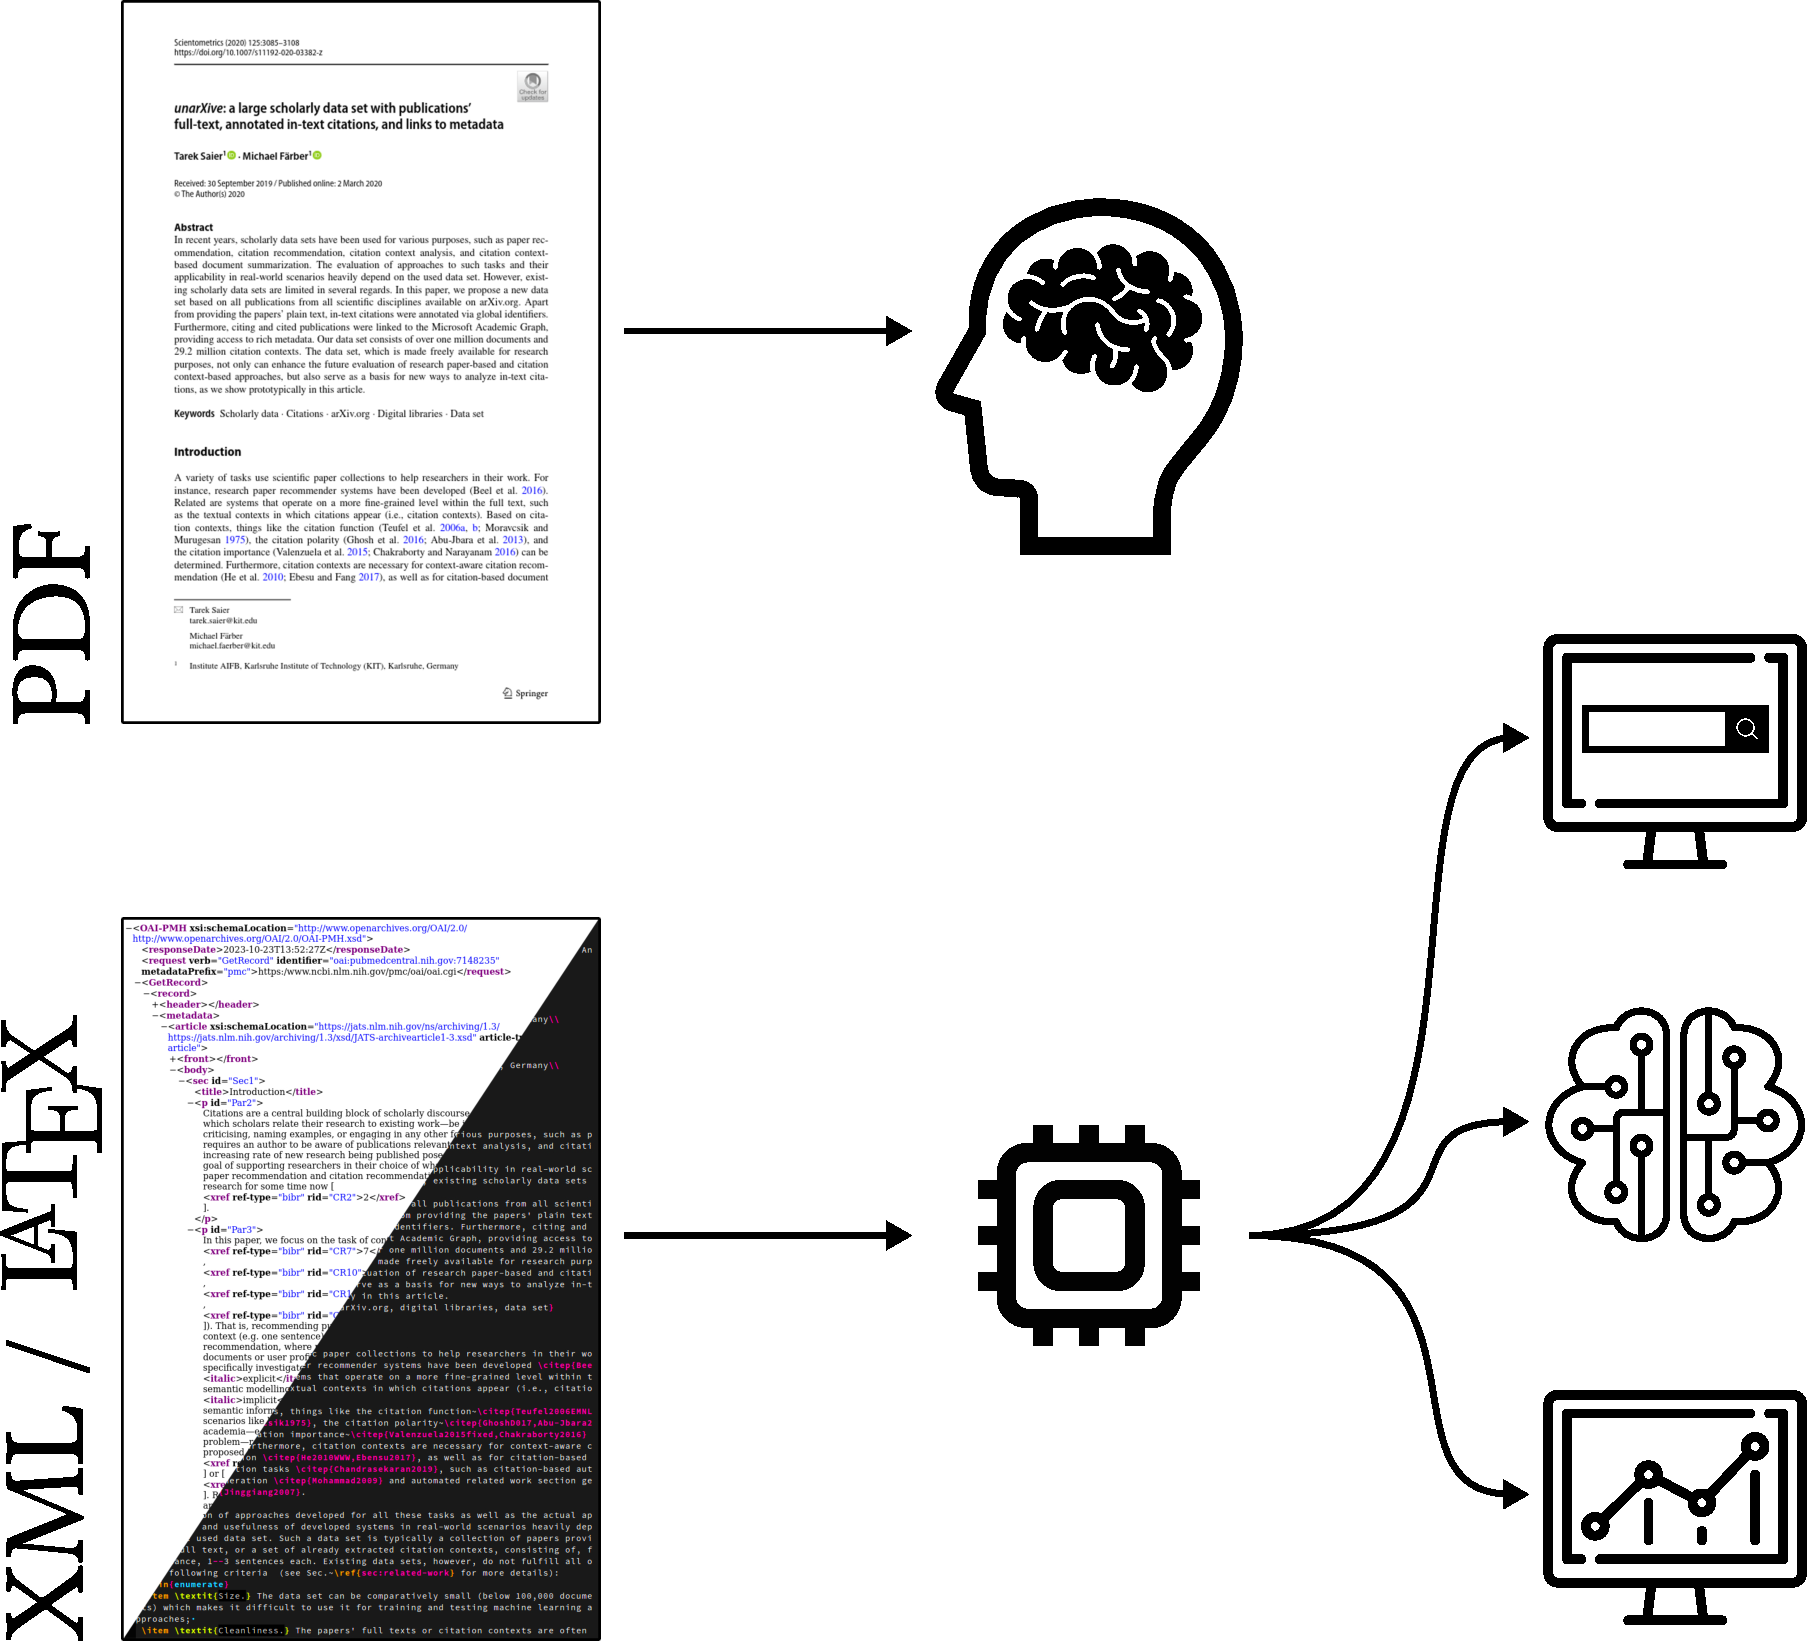
\includegraphics[width=\linewidth]{imgs/scholarly_data_background}
   \end{columns}
   \end{frame}

   \begin{frame}[plain]
        \vspace{0.7cm}
        \begin{infobox-map}
        \centering
        \begin{Huge}
        \textbf{Analogy}\\
        \end{Huge}
        \end{infobox-map}
   \end{frame}

   \begin{frame}{Maps of the Sea}
       \begin{overprint}
           \onslide<1> \centering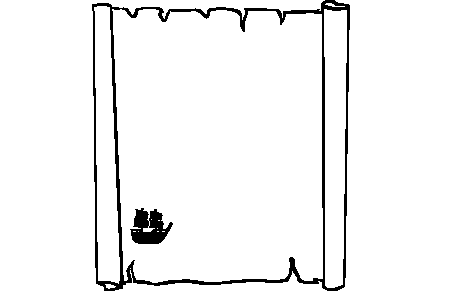
\includegraphics[width=0.55\textwidth]{imgs/schema_analogy_00}
           \onslide<2> \centering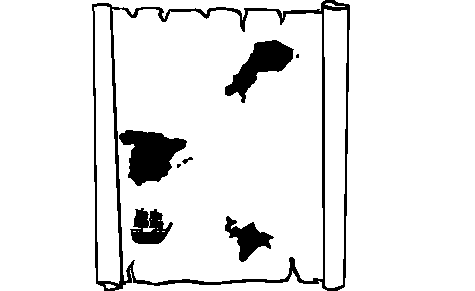
\includegraphics[width=0.55\textwidth]{imgs/schema_analogy_01}
           \onslide<3> \centering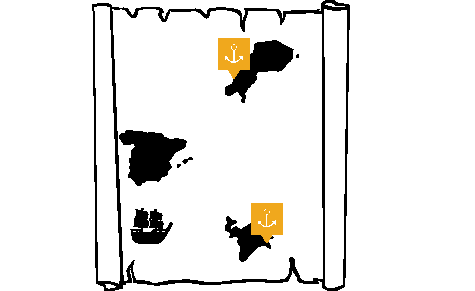
\includegraphics[width=0.55\textwidth]{imgs/schema_analogy_02}
           \onslide<4> \centering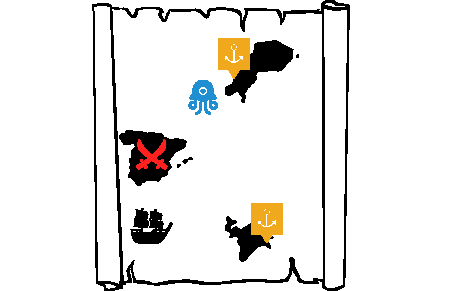
\includegraphics[width=0.55\textwidth]{imgs/schema_analogy_03}
           % TODO: mby insert frame w/ sailor colleagues "discoveing" new islands
           \onslide<5> \centering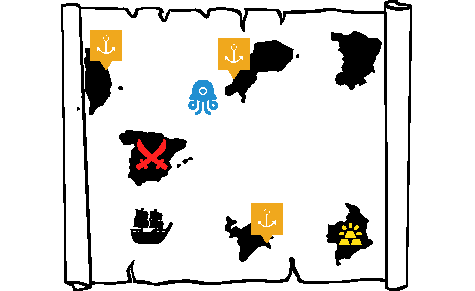
\includegraphics[width=0.55\textwidth]{imgs/schema_analogy_04}
       \end{overprint}
   \end{frame}

   \begin{frame}[t]{Maps of the Sea / Maps of Science}
   \begin{overprint}
    \onslide<1>
       \begin{columns}[t]
           \column{.475\textwidth}
               {\large\textbf{The Sailor} looks for}
               \begin{itemize}
                   \item Port to trade
                   \item Island to explore
               \end{itemize}
           \column{.475\textwidth}
               {\large\textbf{The Scientist} looks for}
               \begin{itemize}
                   \item Paper to read
                   \item Venue to publish at
                   \item Research idea to explore
               \end{itemize}
       \end{columns}
    \onslide<2->
       \begin{columns}
           \column{.475\textwidth}
               {\large\textbf{The Trade Company} looks for}
               \begin{itemize}
                   \item Routes to expand
                   \item Ports to build
                   \item Sailor to hire
               \end{itemize}
           \column{.475\textwidth}
               {\large\textbf{The University/Funding Body} looks for}
               \begin{itemize}
                   \item Research to fund
                   \item Researcher to hire
                   \item Policy to establish
               \end{itemize}
       \end{columns}
   \end{overprint}
    \vspace{1cm}
    \centering
   \only<3>{
        {\Large\textbf{better maps $\Rightarrow$ better decisions}} % \footnote{Abstract representations of the real world}
   }
   \only<4>{
        {\Large\textbf{false maps $\Rightarrow$ misleading/false analyses, models, etc.}}
   }
   \only<5>{
        {\Large\textbf{our maps of science are insufficient}}
   }
   \only<6>{
       \begin{infobox-objective}
       \large\textbf{Research Objective}\\Develop methods for generating large-scale, high quality scholarly data.
       \end{infobox-objective}
   }
   \end{frame}

\section{Background}

   \begin{frame}[plain]
        \vspace{1cm}
        \centering
        \begin{Large}
        {\color{lightgrey}\textbf{Data Mining and Information Extraction Methods}}\\
        \vspace{0.25em}
        {\color{lightgrey}\textbf{for}}\textbf{ Large-Scale High Quality}\\
        \vspace{0.5em}
        {\color{lightgrey}\textbf{Representations of Scientific Publications}}
        \end{Large}
   \end{frame}

   \begin{frame}{Maps of Science}
       \begin{overprint}
           \onslide<1> \centering
\includegraphics[width=0.55\textwidth]{imgs/schema_add_00}
           \onslide<2> \centering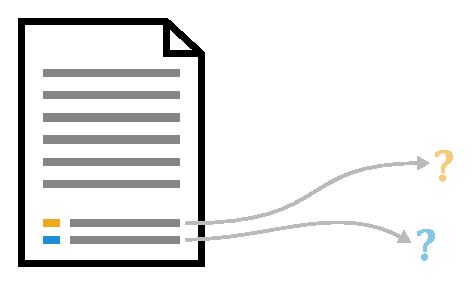
\includegraphics[width=0.55\textwidth]{imgs/schema_add_01}
           \onslide<3> \centering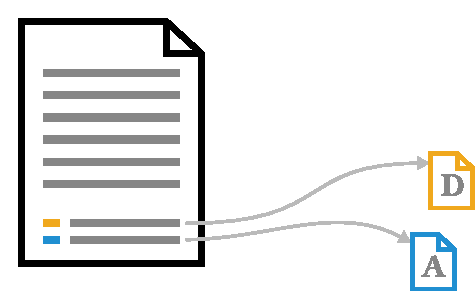
\includegraphics[width=0.55\textwidth]{imgs/schema_add_02}
           \onslide<4> \centering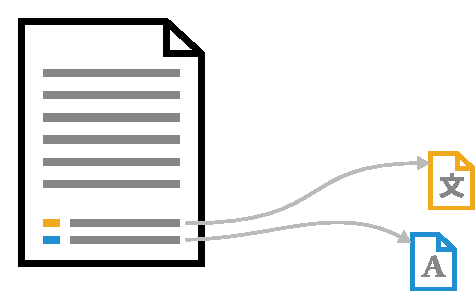
\includegraphics[width=0.55\textwidth]{imgs/schema_add_03}
           \onslide<5> \centering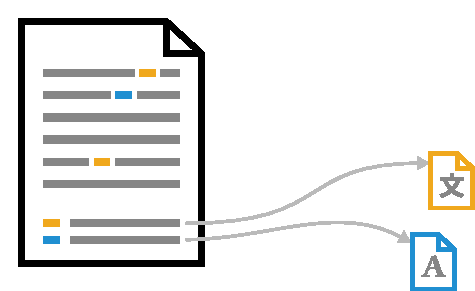
\includegraphics[width=0.55\textwidth]{imgs/schema_add_04}
           \onslide<6> \centering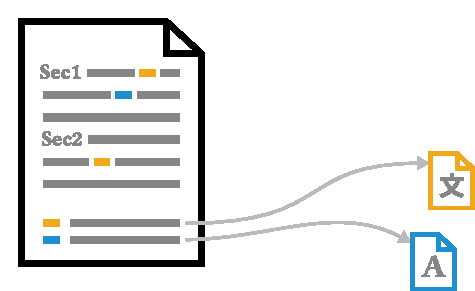
\includegraphics[width=0.55\textwidth]{imgs/schema_add_05}
           \onslide<7> \centering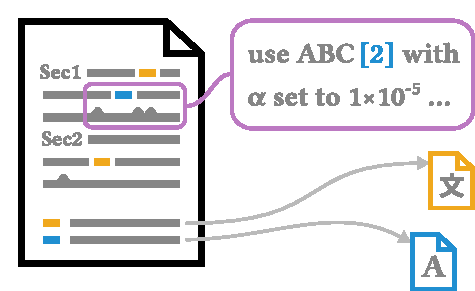
\includegraphics[width=0.55\textwidth]{imgs/schema_add_06}
           \onslide<8> \centering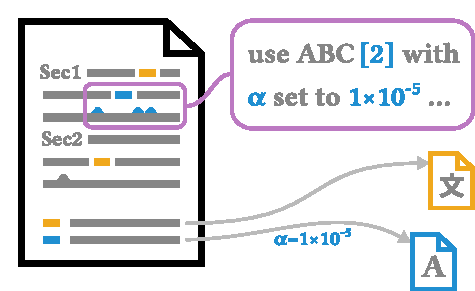
\includegraphics[width=0.55\textwidth]{imgs/schema_add_07}
           \onslide<9> \centering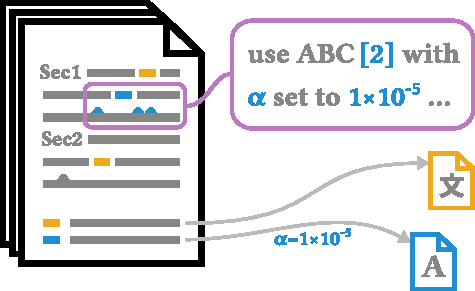
\includegraphics[width=0.55\textwidth]{imgs/schema_add_08}
           \onslide<10> \centering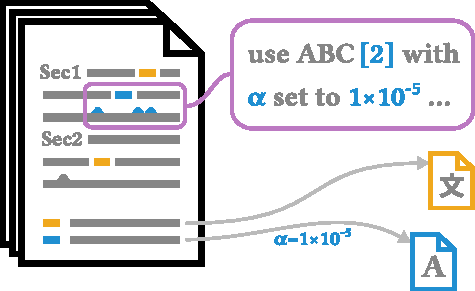
\includegraphics[width=0.55\textwidth]{imgs/schema_add_09}
       \end{overprint}
   \end{frame}

   \begin{frame}
       \frametitle<1-2>{Research Gap: Citation Network}
       \frametitle<3-6>{Research Gap: Non-English Documents}
       \frametitle<7-8>{Research Gap: Artifact Parameters}
       \begin{overprint}
           % visualize research gaps
           \onslide<1> \centering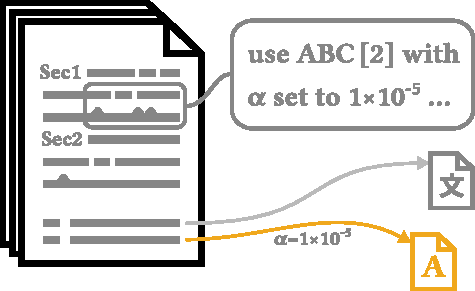
\includegraphics[width=0.55\textwidth]{imgs/schema_add_09_vargapcit_0}
           \onslide<2> \centering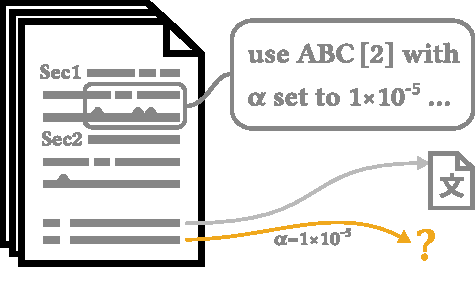
\includegraphics[width=0.55\textwidth]{imgs/schema_add_09_vargapcit_1}
           % - Gap: Citation Network
           % - Vis: Doc A to question mark
           % - Importance: prevalent use cases hinge on cn
           \onslide<3> \centering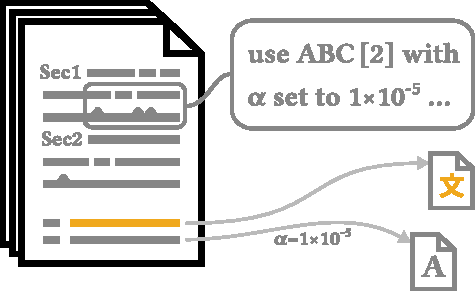
\includegraphics[width=0.55\textwidth]{imgs/schema_add_09_vargapling_0}
           \onslide<4> \centering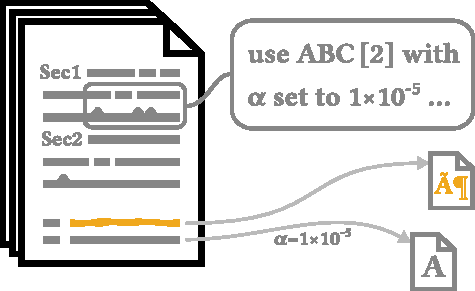
\includegraphics[width=0.55\textwidth]{imgs/schema_add_09_vargapling_1}
           \onslide<5> \centering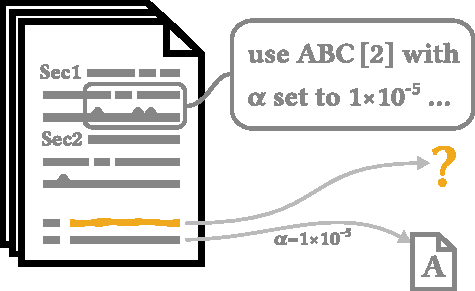
\includegraphics[width=0.55\textwidth]{imgs/schema_add_09_vargapling_2}
           \onslide<6> \centering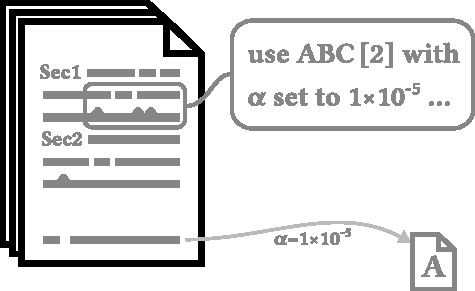
\includegraphics[width=0.55\textwidth]{imgs/schema_add_09_vargapling_3}
           % - Gap: Anglocentrism
           % - Vis: Doc 文 and refsecentry first 文字化け, then disappear
           % - Importance: science is a global = multi-lingual endeavor
           \onslide<7> \centering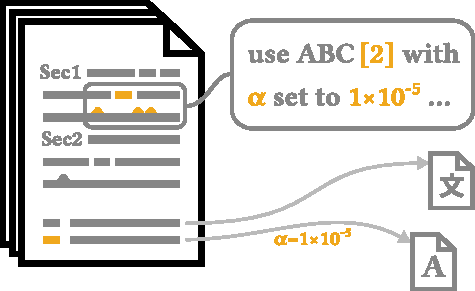
\includegraphics[width=0.55\textwidth]{imgs/schema_add_09_vargapartf_0}
           \onslide<8> \centering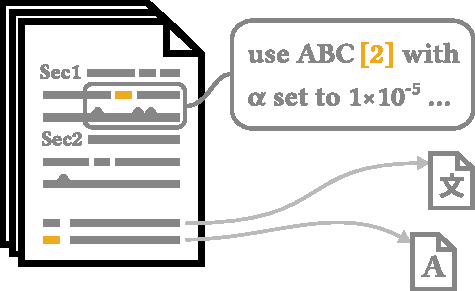
\includegraphics[width=0.55\textwidth]{imgs/schema_add_09_vargapartf_1}
           % - Gap: Research Artifacts
           % - Vis: Text bumps, blue highlights, cit param disappear
           % - Importance: increasingly a research driver
       \end{overprint}
   \end{frame}

   \begin{frame}[plain]
        \vspace{1cm}
        \centering
        \begin{Large}
        \textbf{Data Mining and Information Extraction Methods}\\
        \vspace{0.25em}
        {\color{lightgrey}\textbf{for Large-Scale High Quality}}\\
        \vspace{0.5em}
        {\color{lightgrey}\textbf{Representations of Scientific Publications}}
        \end{Large}
   \end{frame}

\section{Outline}

   \begin{frame}[plain]
       \begin{overprint}
           \onslide<1> \centering
\includegraphics[width=\textwidth]{imgs/objective_grid_and_contrib_0}
           \onslide<2> \centering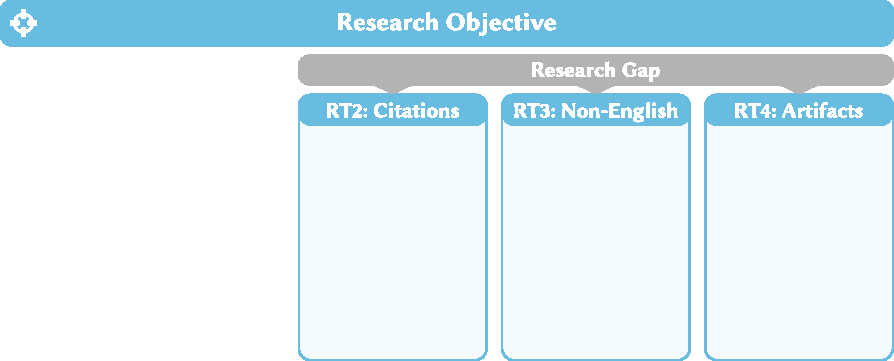
\includegraphics[width=\textwidth]{imgs/objective_grid_and_contrib_1}
           \onslide<3> \centering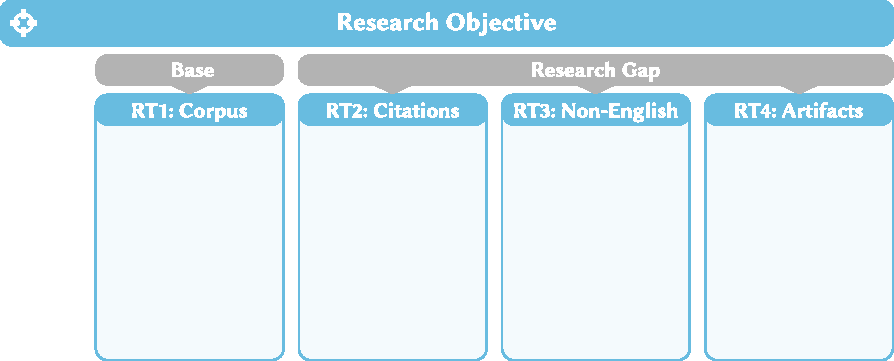
\includegraphics[width=\textwidth]{imgs/objective_grid_and_contrib_2}
           \onslide<4> \centering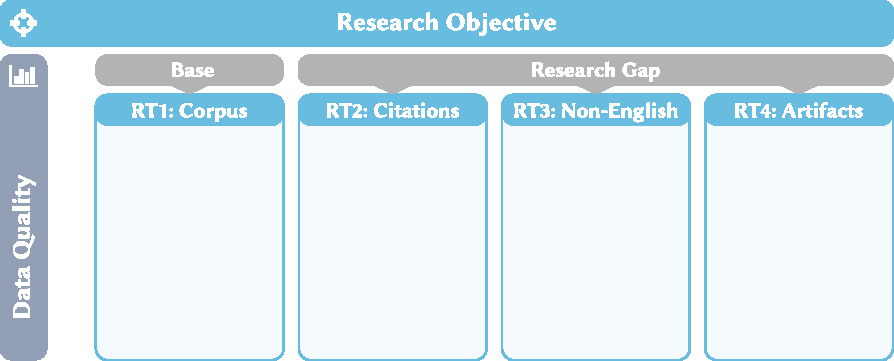
\includegraphics[width=\textwidth]{imgs/objective_grid_and_contrib_3}
           \onslide<5> \centering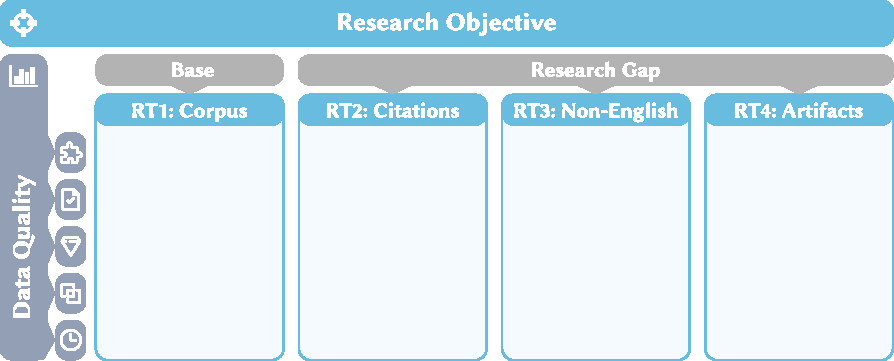
\includegraphics[width=\textwidth]{imgs/objective_grid_and_contrib_4}
           \onslide<6> \centering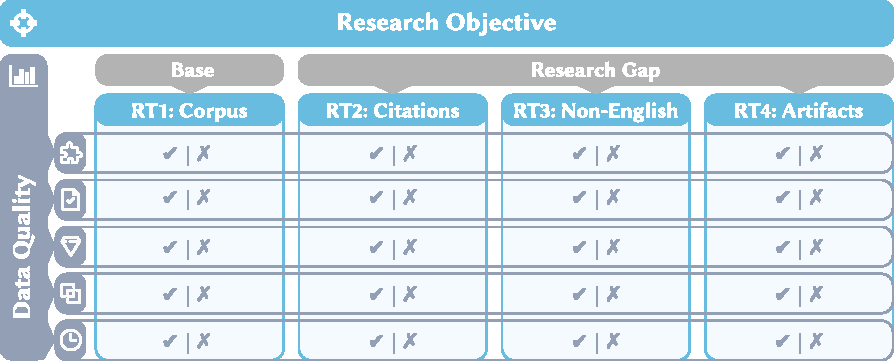
\includegraphics[width=\textwidth]{imgs/objective_grid_and_contrib_5}
           \onslide<7> \centering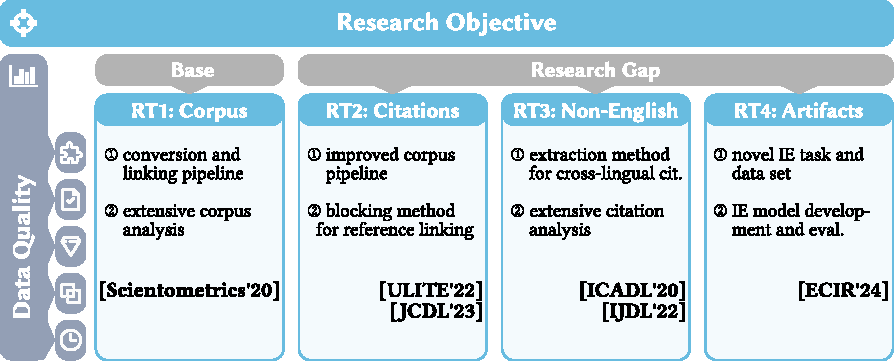
\includegraphics[width=\textwidth]{imgs/objective_grid_and_contrib_6}
           \onslide<8> \centering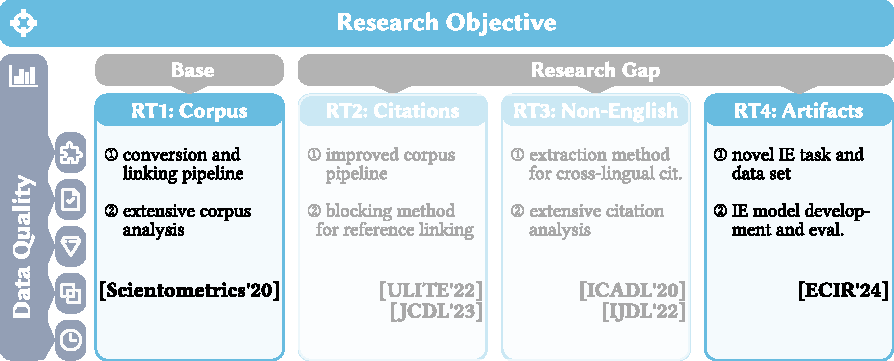
\includegraphics[width=\textwidth]{imgs/objective_grid_and_contrib_7}
       \end{overprint}
   \end{frame}

   % - why is this challenging?
   % - what is the benefit/necessity?

   % \begin{frame}{Challenges}
   %     \begin{infobox-discussion}
   %     \textbf{Discussion} Human made in the first place, so why not already fit for our needs?
   %     \end{infobox-discussion}

   %     \begin{itemize}
   %         \item Historical baggage
   %         \item Made for human consumption
   %         \item Primarily visual
   %     \end{itemize}
   % \end{frame}

   % \begin{frame}[plain]
   %     \vspace{1.25cm}
   %     \begin{overprint}
   %         \onslide<1> \centering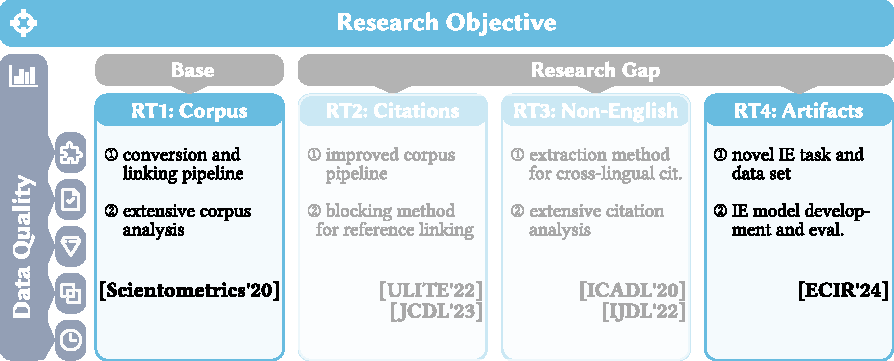
\includegraphics[width=0.85\textwidth]{imgs/objective_grid_and_contrib_7}
   %     \end{overprint}
   % \end{frame}

   % \begin{frame}[plain]
   %      \vspace{0.7cm}
   %      \begin{infobox-map}
   %      \centering
   %      \begin{Huge}
   %      \textbf{Outline}\\
   %      \end{Huge}
   %      \end{infobox-map}
   % \end{frame}

   \begin{frame}{Outline}
   \begin{columns}
       \column{.3\textwidth}
           \begin{itemize}
               \item \textbf{Corpus}
               \begin{itemize}
                   \item Challenges
                   \item Solutions
                   \item Resulting Corpus
               \end{itemize}
               \item {\color{contextgrey}\textbf{Citation Network}}
               \item {\color{contextgrey}\textbf{Non-English Documents}}
               \item \textbf{Artifact Parameters}
               \begin{itemize}
                   \item Task Definition
                   \item Methods
                   \item Results
               \end{itemize}
               \item \textbf{Conclusion}
               \begin{itemize}
                   \item Contributions
                   \item Impact
               \end{itemize}
           \end{itemize}
       \column{.575\textwidth}
            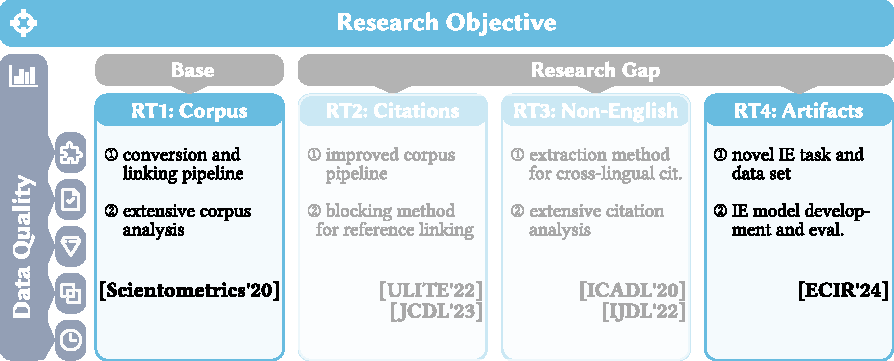
\includegraphics[width=\linewidth]{imgs/objective_grid_and_contrib_7}
   \end{columns}
   \end{frame}

   % \begin{frame}{Research Questions}
   %     \begin{infobox-q}
   %     \textbf{RQ1} How can the completeness of the citation network in scholarly data sets be improved?
   %     \end{infobox-q}

   %     \begin{infobox-q}
   %     \textbf{RQ2} How can the completeness of the citation network in scholarly data sets be improved?
   %     \end{infobox-q}

   %     \begin{infobox-info}
   %     \textbf{Remark} This text should show what a printed text will look like at this place. If you read this text, you will get no information. Really? Is there no information?
   %     \end{infobox-info}
   % \end{frame}

   % \begin{frame}{Contributions}
   %     \begin{infobox-pub}
   %     \begin{scriptsize}
   %     \textbf{Publication} \fullcite{Saier2020}
   %     \end{scriptsize}
   %     \end{infobox-pub}

   %     \begin{infobox-pub-small}
   %     \textbf{Scientometrics'20}~\cite{Saier2020}
   %     \end{infobox-pub-small}
   %     \begin{infobox-pub-small}
   %     \textbf{IJDL'21}~\cite{Saier2021}
   %     \end{infobox-pub-small}

   %     \begin{itemize}
   %         \item to achive this (four aspects shown before),
   %         \begin{itemize}
   %         \item (show image w/ unarXive as base/roof)
   %         \item created data set, using this data set, developed methods to
   %         \item improve (general) reference completeness and content granularity
   %         \item improve completness of and analyze references to different languages
   %         \item enable IE for fine (re-)use w/ parameters
   %         \end{itemize}
   %     \end{itemize}
   % \end{frame}

\section{Corpus}

   \begin{frame}[plain]
        \vspace{0.7cm}
        \begin{infobox-map}
        \centering
        \begin{Huge}
        \only<1> {\textbf{Corpus}}
        \only<2> {\textbf{\hphantom{C}unarXive\hphantom{C}}}
        \end{Huge}
        \end{infobox-map}
   \end{frame}

   \begin{frame}{Corpus - Digest}
   \begin{columns}
       \column{.575\textwidth}
        \begin{itemize}
            \item \textbf{Research Task}\\Develop a method for creating large-scale, high quality ``base corpus''
            \item \textbf{Method}
            \begin{itemize}
                \item Conversion of / IE from \LaTeX
                \item Joint handling of text + references
                \item Reference parsing + linking to metadata records
            \end{itemize}
            \item \textbf{Results}
            \begin{itemize}
                \item Corpus among 3 largest full-text corpora
                \item More extensive, complete, less noisy data
                \item State of the art reference linking
            \end{itemize}
        \end{itemize}
        % \begin{itemize}
        %     \item \textbf{Research gap}
        %     \begin{itemize}
        %         \item Corpus size
        %         \item Data cleanliness
        %         \item Reference linking
        %     \end{itemize}
        %     \item \textbf{Approach}
        %     \begin{itemize}
        %         \item Joint handling of text + references
        %         \item Conversion of / IE from \LaTeX
        %         \item Reference parsing + linking to metadata records
        %     \end{itemize}
        %     \item \textbf{Results}
        %     \begin{itemize}
        %         \item Corpus creation methodology
        %         \item More extensive, complete; less noisy data
        %         \item Large corpus for further research
        %     \end{itemize}
        % \end{itemize}
       \column{.375\textwidth}
            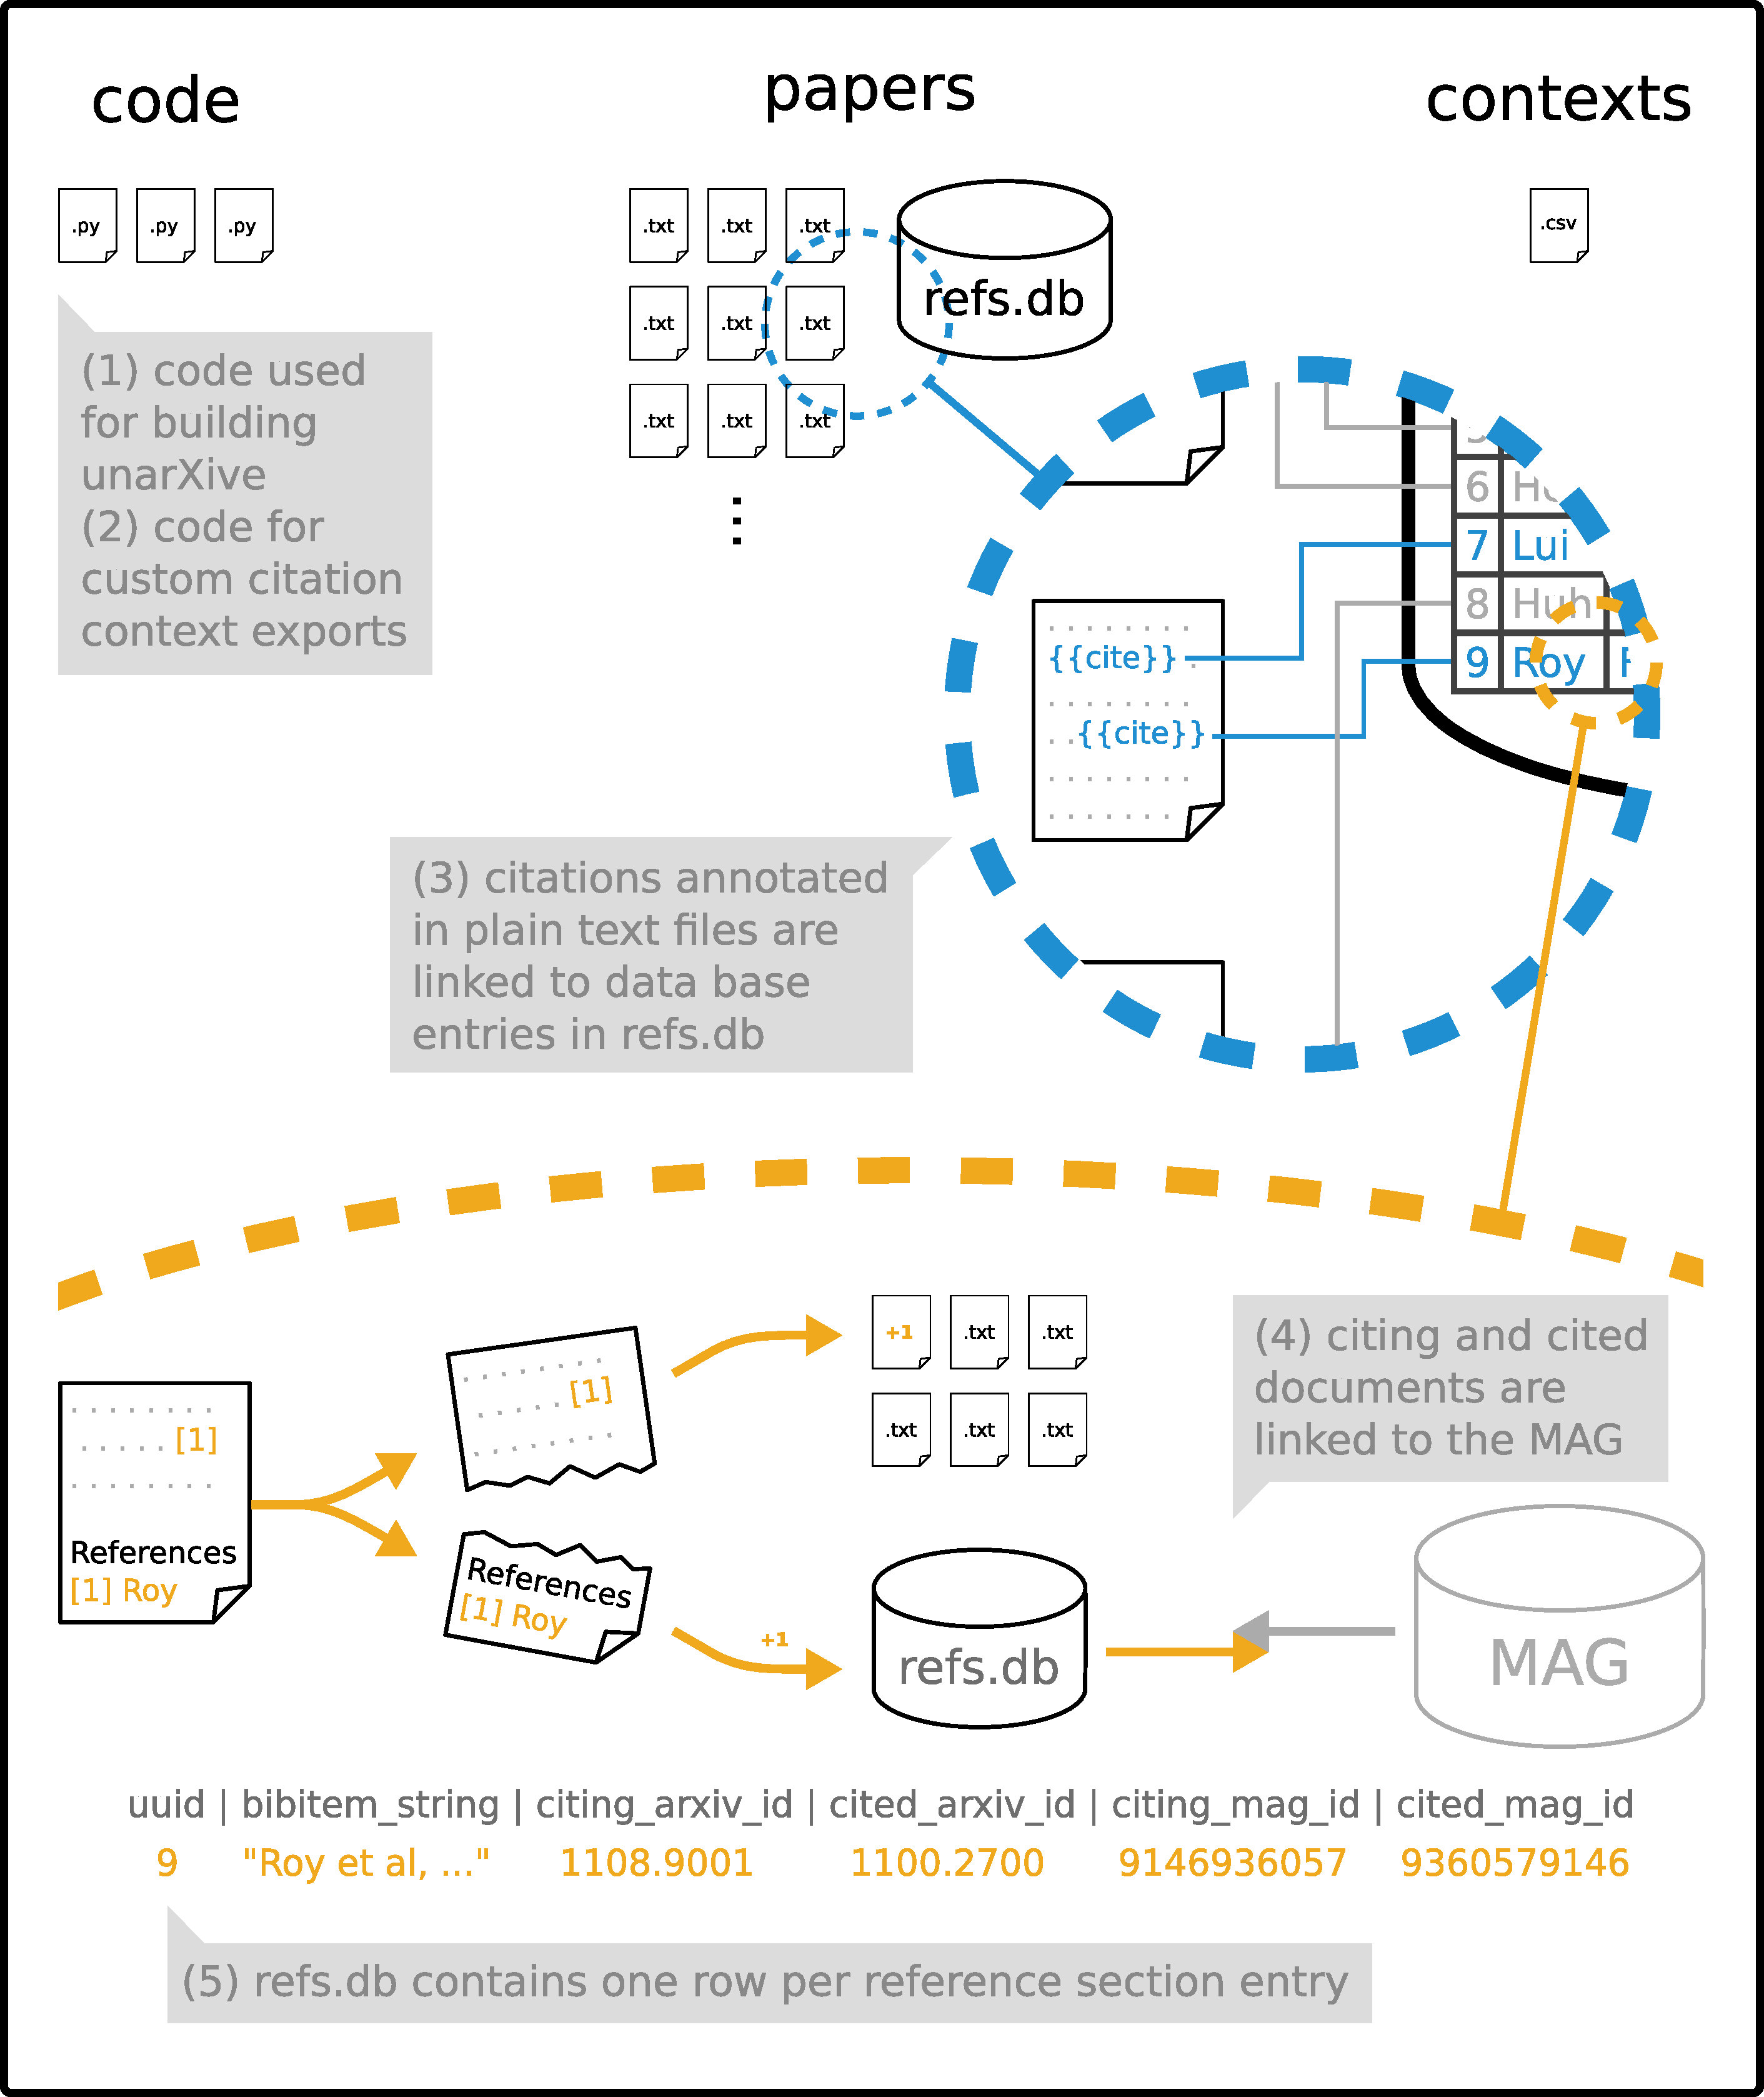
\includegraphics[width=0.75\linewidth]{imgs/unarXive_2020_structure_with_db}
           \begin{infobox-pub-small}
           \textbf{Scientometrics'20}~\cite{Saier2020}
           \end{infobox-pub-small}
   \end{columns}
   \end{frame}

   % \begin{frame}{Corpus - Pipeline}
   %  \centering
   %  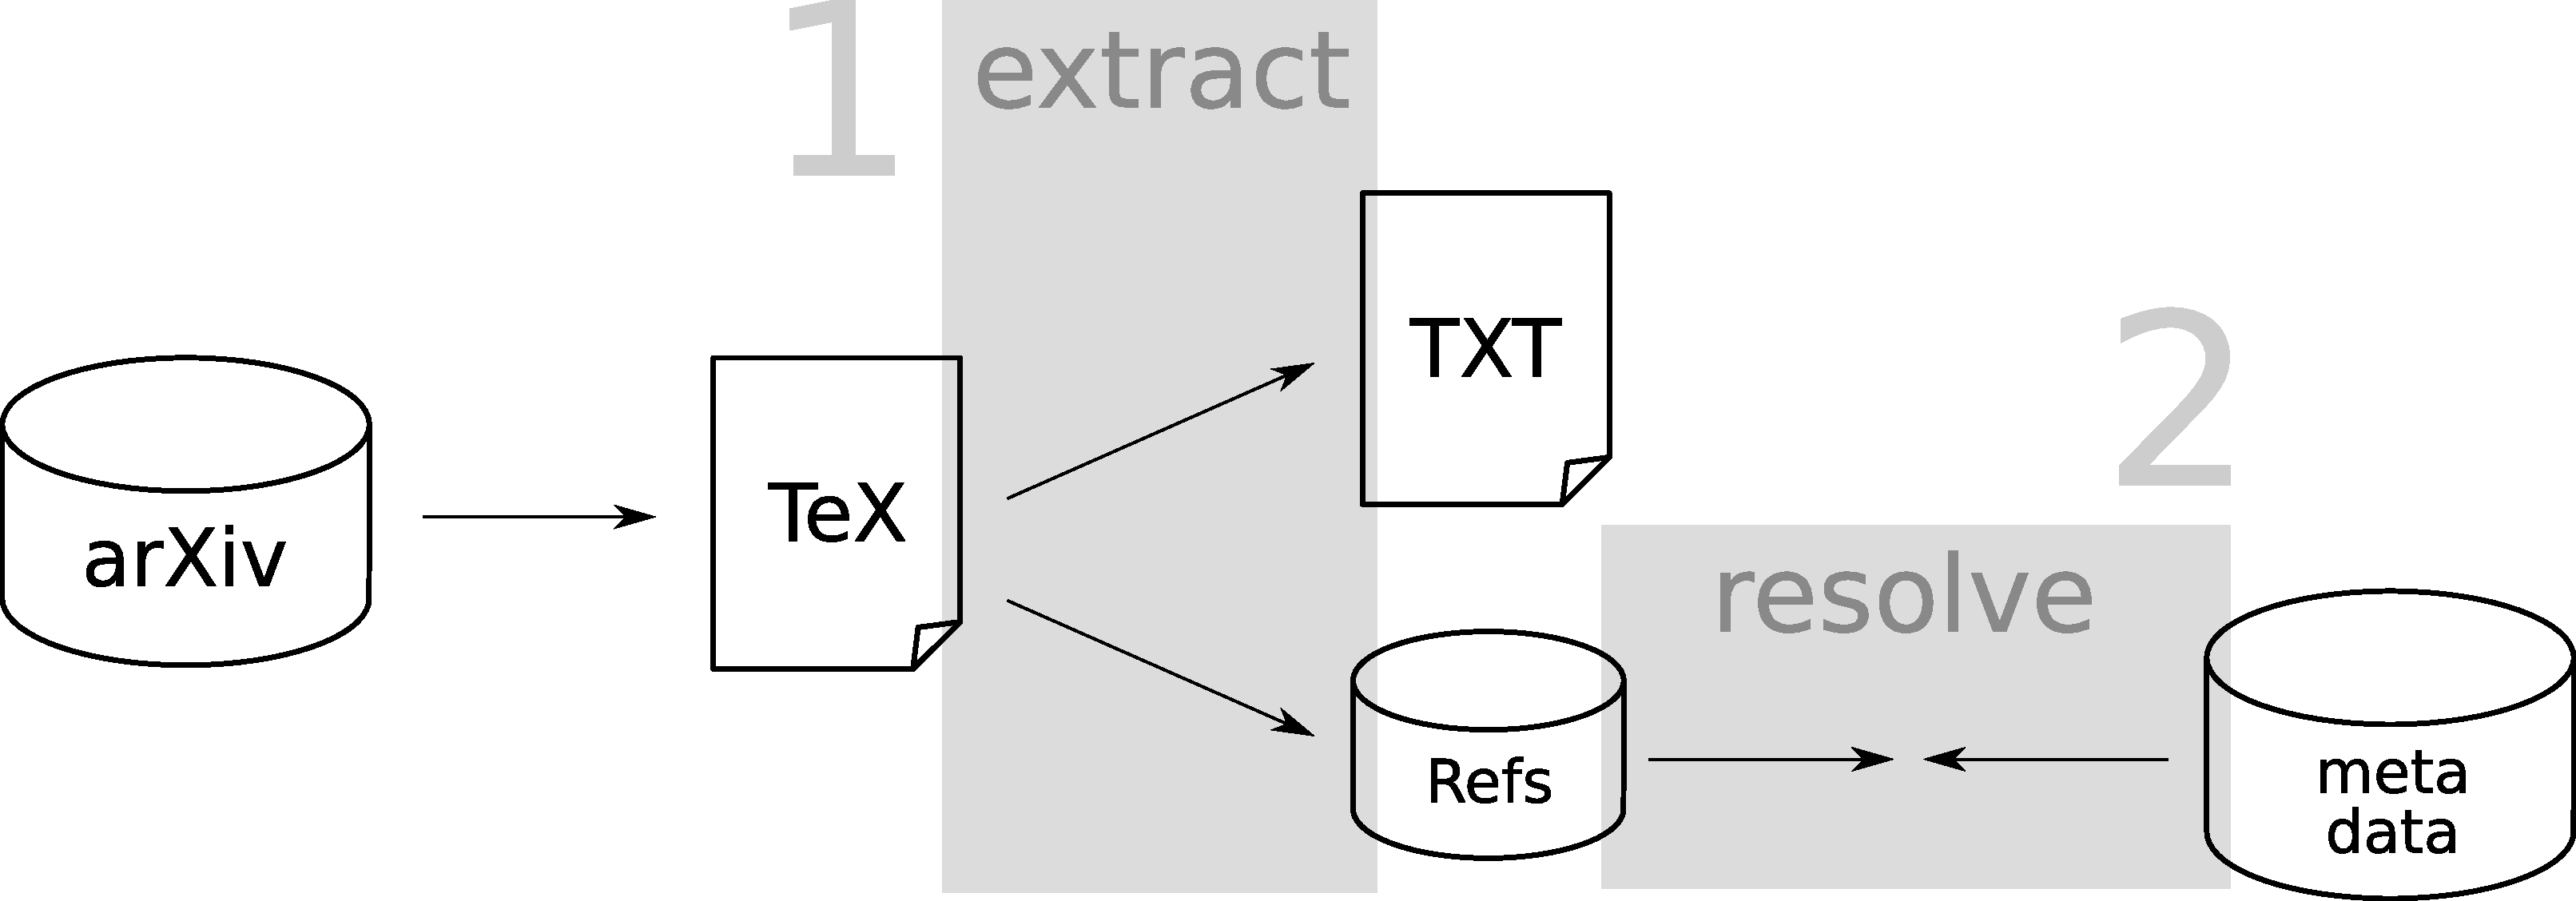
\includegraphics[width=.7\textwidth]{imgs/data_set_generation_schema_simple.pdf}
   % \end{frame}

   \begin{frame}{Corpus - Challenges}
   \begin{columns}
       \column{.575\textwidth}
        \begin{itemize}
            \item \textbf{General}
            \begin{itemize}
                \item Volume ($\sim10^6$ docs, $\sim10^7$ refs)
                \item Bridging visual medium and text information  % (e.g. footnotes: how to incorporate? Special syntax? Keep LaTeX as is? -- what about bold and italic text? Keep? ...)
            \end{itemize}
            \item \textbf{Parsing}
            \begin{itemize}
                \item Parser efficiency
                \item Typesetting info $\neq$ semantic info
                \item \LaTeX{} is powerful and people are creative
            \end{itemize}
            \item \textbf{Reference linking}
            \begin{itemize}
                \item Choice of target set
                \item Parsing (\texttt{bbl}, not \texttt{bib})
                \item Variance and information sparsity
            \end{itemize}
        \end{itemize}
       \column{.475\textwidth}
          \centering
          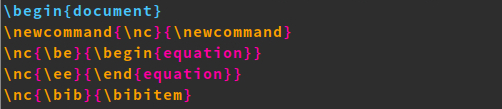
\includegraphics[width=0.8\linewidth]{imgs/renewcommand}

          \vspace{0.5cm}
          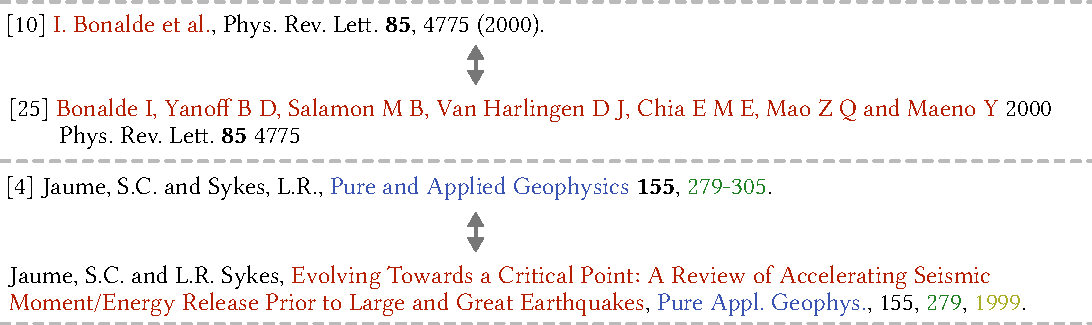
\includegraphics[width=\linewidth]{imgs/hardmatch_examples}
   \end{columns}
   \end{frame}

   \begin{frame}{Corpus - Solutions}
    \centering
    \only<1>{
    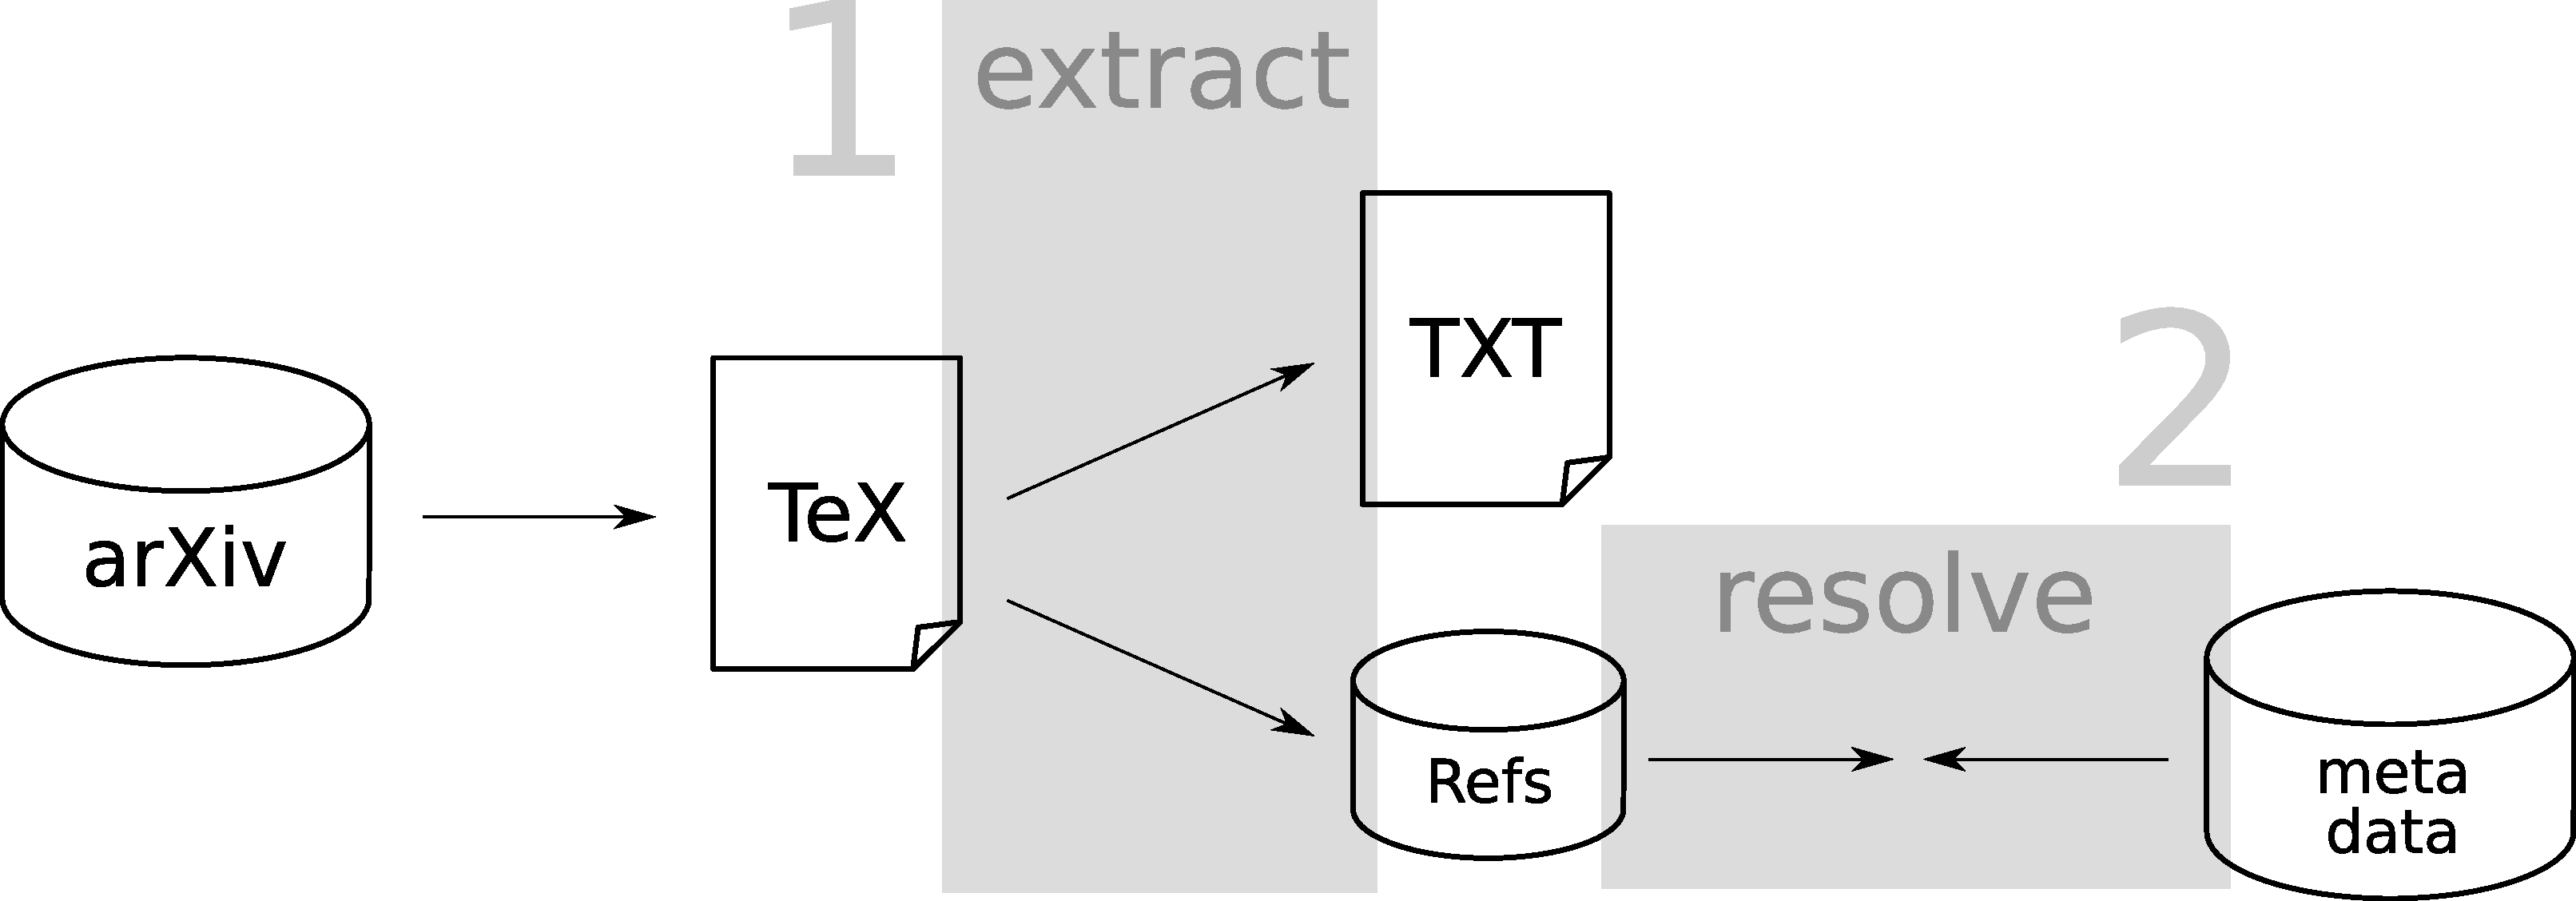
\includegraphics[width=.7\textwidth]{imgs/data_set_generation_schema_simple.pdf}
    }
    \only<2>{
    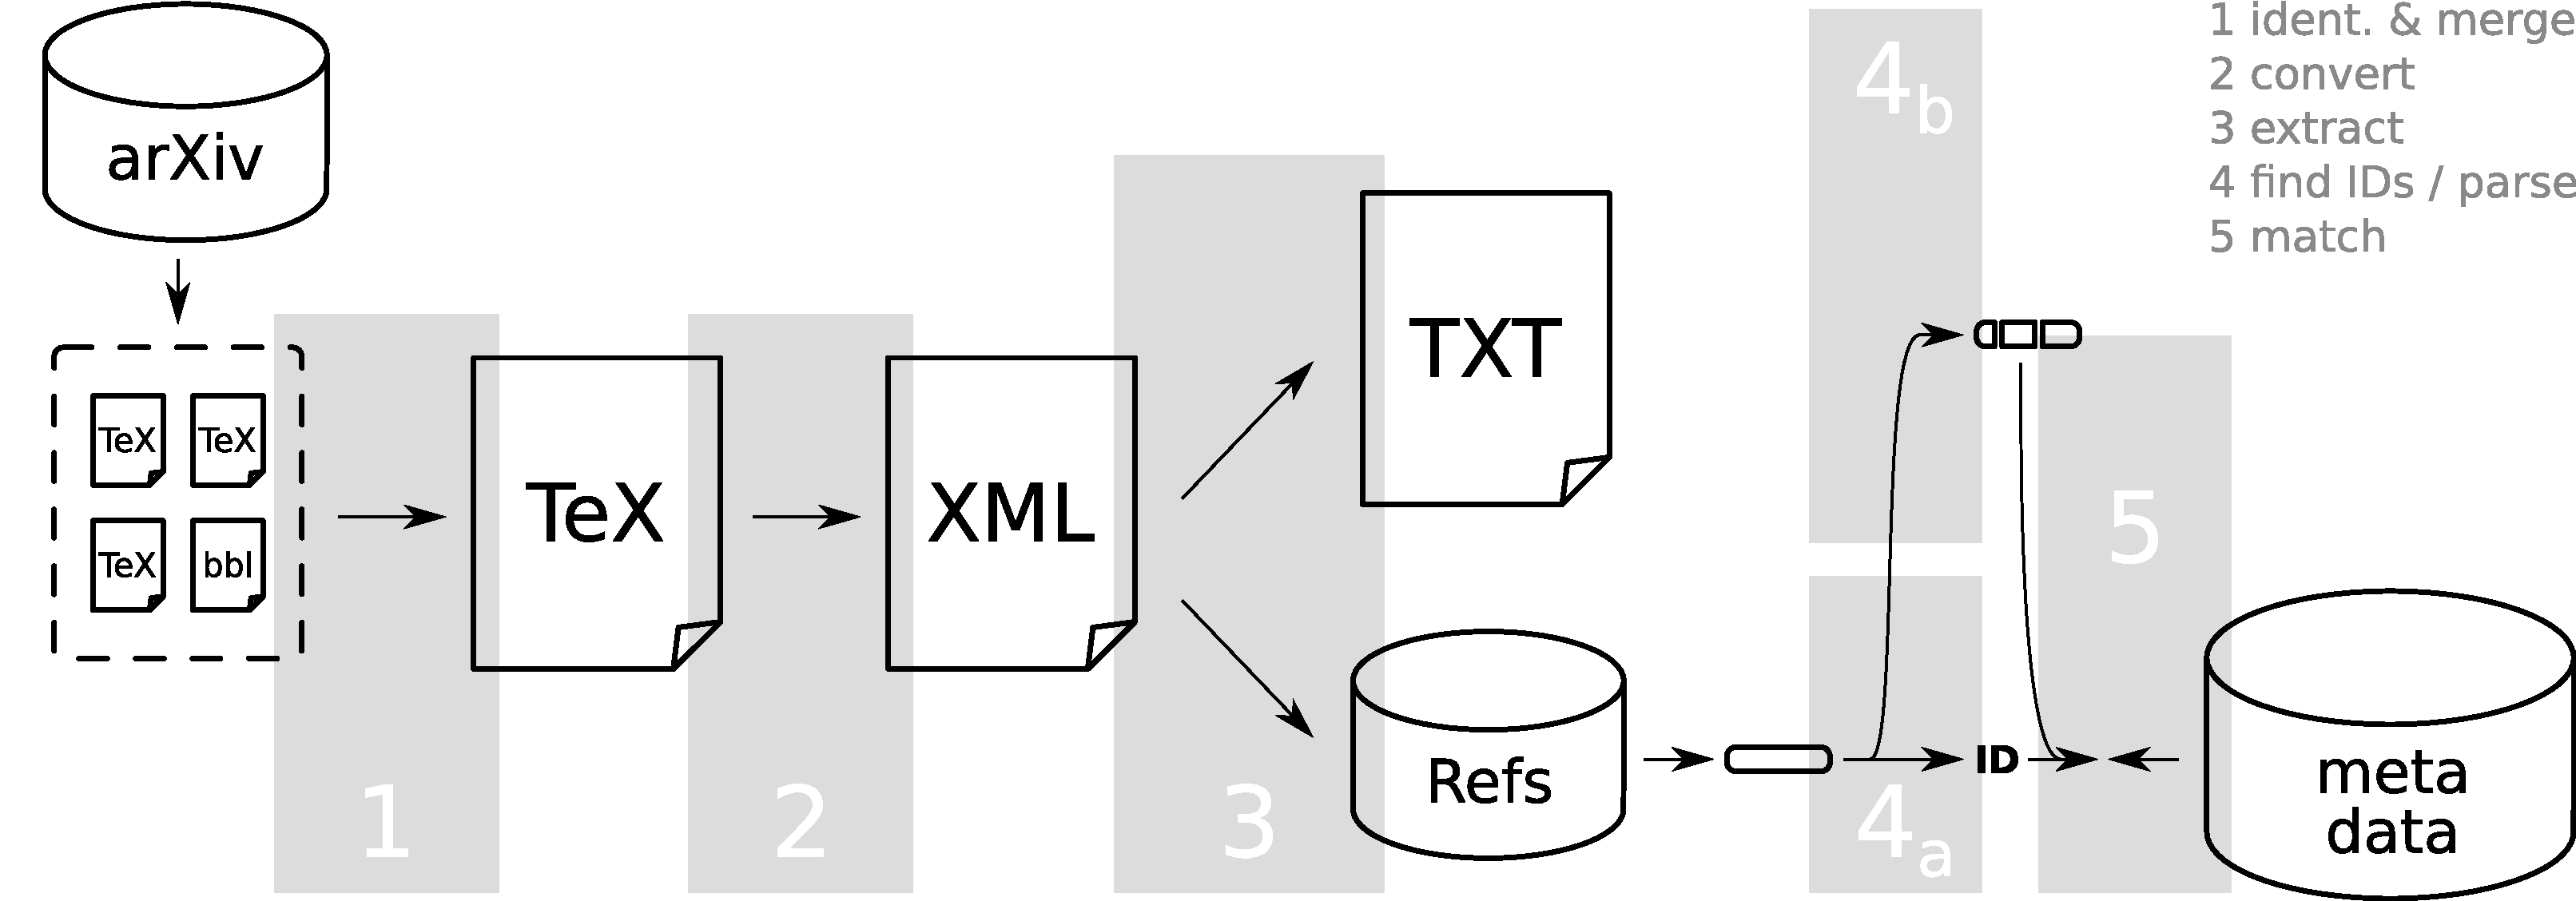
\includegraphics[width=.7\textwidth]{imgs/data_set_generation_schema_full.pdf}
    }
   \end{frame}

   % \begin{frame}{Corpus - Solutions}
   %  \begin{itemize}
   %      \item \textbf{Parsing}
   %      \begin{itemize}
   %          \item \LaTeX{} $\rightarrow$ XML (Tralics)
   %          \item identify semantically significant content (cit. markers, references, formulae, figures, tables, ...)
   %          \item give IDs and store away
   %          \item identify main text, convert XML to text
   %      \end{itemize}
   %      \item \textbf{Reference linking}
   %      \begin{itemize}
   %          \item chose MAG (/OpenAlex) as target set, local dump in indexed DB
   %          \item find potential identifiers (DOI, arXiv), use if present (DOI: crossref, arXiv: metadata dump)
   %          \item parse otherwise (NeuralParscit)
   %          \item match based on title and author(s) (unified normalization, dealing with duplicates in target set)
   %      \end{itemize}
   %  \end{itemize}
   % \end{frame}

   \begin{frame}{Corpus - Result}
   \begin{columns}
       \column{.575\textwidth}
        \begin{itemize}
            \item \textbf{Size}
            \begin{itemize}
                \item 1.2\,M documents (2.7\,M cited)
                \item 16\,M references
                \item 29\,M in-text citation markers
            \end{itemize}
            \item \textbf{Scope}
            \begin{itemize}
                \item 1991--2018 (current: 2022)
                \item physics (63\%), maths (23\%), CS (11\%), other (3\%)
            \end{itemize}
            \item \textbf{Reference matching}
            \begin{itemize}
                \item 53\% by parsing + matching
                \item 28\% by DOI
                \item 19\% by arXiv ID
            \end{itemize}
        \end{itemize}
       \column{.375\textwidth}
            %\includegraphics[width=0.75\linewidth]{imgs/}
   \end{columns}
   \end{frame}

   \begin{frame}{Corpus - Result}
    % - stats
    % - novel analyses
    % - (usage by community?) — mby better at the very end

    \begin{table}
     %\caption{Existing data sets}  %\\\small{(\#P.=Number of papers; Cit.\ cont.=Citation contexts; Ref.\ IDs=Reference IDs; CS=Computer Science, BM=Biomedicine, LS=Life Sciences, CL=Computer Linguistics)\\(\emph{extractable*} indicates that extraction might be error-prone due to papers only being available in PDF format)}}
     %\label{tab:existing-data-sets}
      \centering
      \begin{small}
     \begin{threeparttable}
     \begin{tabular}{lccccc}
     \toprule
       Data set & \# Docs & Cit. markers & Disciplines & Full text & Linked \\
       \midrule
       % capital Ms and lowercase ks (supposed to be like that)
       ACL-ARC~\cite{Bird2008ACLARC} & 11 k & no & comp. ling. & PDF & $\times$ \\
       ACL-AAN~\cite{Radev2013} & 18 k & no & comp. ling. & PDF & $\times$  \\
       Scholarly Dataset 2~\cite{Sugiyama2015} & 100 k & no & CS & PDF & $\times$ \\
       CiteSeerX~\cite{Caragea2014} / RefSeer~\cite{Huang2015fixed} &  1 M & ambiguous & mixed & 400 char excerpts & $\times$ \\
       PMC OAS~\cite{pmc_oas} & 2.3 M & exact & biomedical & XML & mixed\tnote{a} \\
       arXiv CS~\cite{Faerber2018LREC}   &  90 k & exact & CS & text & \checkmark \\
       \textbf{unarXive}~\cite{Saier2020} & 1.2 M & exact & phys., maths, CS & text & \checkmark \\
       \bottomrule
     \end{tabular}
     \begin{tablenotes}
        \item[a] {\color{contextgrey}No citation network due to mixed set of IDs (PubMed, MEDLINE, DOI)~\cite{Gipp2015}.}
      \end{tablenotes}
    \end{threeparttable}
      \end{small}
    \end{table}
   \end{frame}


   \begin{frame}{Corpus - Result (2022)}
    \begin{table}
      % \caption[Comparison of large data sets derived from paper full-texts]{Comparison of large data sets derived from paper full-texts ($^\dagger$Cit. network completeness is reported is two ways. ``general'': the whole data set; not directly comparable. ``compare'': for arXiv.org data from 1991--2020; directly comparable. $^\ddagger$References in the PMC-OAS are partially linked to a mixed set of IDs (PubMed, MEDLINE, DOI)~\cite{Gipp2015}. Therefore there is no single, comprehensive number for its completeness.}
      % \label{tab:comparison}
      \centering
      \begin{small}
     \begin{threeparttable}
      \begin{tabular}{lcccccc}
        \toprule
        \ & \multicolumn{2}{c}{Source} & \multicolumn{2}{c}{\hphantom{wi}Citation Network\tnote{a}} & \ & \ \\
        Data Set & Data & Format & general & compare & \# Docs & Disciplines \\
        \midrule
        CORE~\cite{core} & multiple & PDF & 0\% & - & $>$100 M & various \\
        S2ORC (PDF)~\cite{Lo2020} & multiple & PDF & 69.4\% & - & 12 M & various \\
        % (19.3+6.8)/(27.8+21.9) = 53% overall, 69.4% GROBID parses, 31.1% LaTeX parses
        unarXive 2020~\cite{Saier2020} & arXiv.org & \LaTeX & 42.6\% & 42.6\% & 1.2 M & phys., maths, CS \\
        \midrule
        S2ORC (\LaTeX)~\cite{Lo2020} & arXiv.org & \LaTeX & 31.1\% & 31.1\% & 1.5 M & phys., maths, CS \\
        arXMLiv~\cite{arXMLiv} & arXiv.org & \LaTeX & 0\% & 0\% & 1.6 M & phys., maths, CS \\
        SciXGen~\cite{chen2021-scixgen} & arXiv.org & \LaTeX & 41.6\% & - & 205 k & CS \\
        PMC-OAS~\cite{pmc_oas} & PubMed & XML & mixed\tnote{b} & - & \textbf{3.3 M} & \textbf{biomedical} \\
        \textbf{unarXive 2022}~\cite{Saier2023unarXive} & arXiv.org & \LaTeX & 44.4\% & \textbf{44.4\%} & \textbf{1.9 M} & \textbf{phys., maths, CS} \\
        % 0.4441 for 1991—2022, 0.4438 for 1991–2020
        \bottomrule
      \end{tabular}
     \begin{tablenotes}
        \item[a] {\color{contextgrey}``general'': all data; incomparable. ``compare'': arXiv.org data 1991--2020; directly comparable.}
        \item[b] {\color{contextgrey}No citation network due to mixed set of IDs (PubMed, MEDLINE, DOI)~\cite{Gipp2015}.}
      \end{tablenotes}
    \end{threeparttable}
      \end{small}
    \end{table}
   \end{frame}

   \begin{frame}{Corpus - Link Correctness}
    \begin{table}[tb]
      \caption{Link correctness (n = 300)}
      \centering
      \begin{small}
     \begin{threeparttable}
    \begin{tabular}{c@{\hspace{0.1in}}c@{\hspace{0.1in}}c@{\hspace{0.1in}}c}
    \toprule
        Confidence level & Method\tnote{a} & Lower limit & Upper limit \\
    \midrule
        0.99 & Wilson & 0.9613 & 0.9975 \\\noalign{\smallskip}
        \ & Jeffreys & 0.9666 & 0.9983 \\\noalign{\smallskip}
        \hline\noalign{\smallskip}
        0.95 & Wilson & 0.9710 & 0.9966 \\\noalign{\smallskip}
        \ & Jeffreys & 0.9736 & 0.9972 \\
        \bottomrule
    \end{tabular}
     \begin{tablenotes}
        \item[a] {\color{contextgrey}Confidence interval given as Wilson score interval and Jeffreys interval~\cite{Brown2001}.}
      \end{tablenotes}
     \end{threeparttable}
    \end{small}
    \end{table}
   \end{frame}

   \begin{frame}{Corpus - Citation Flow}
    \centering
    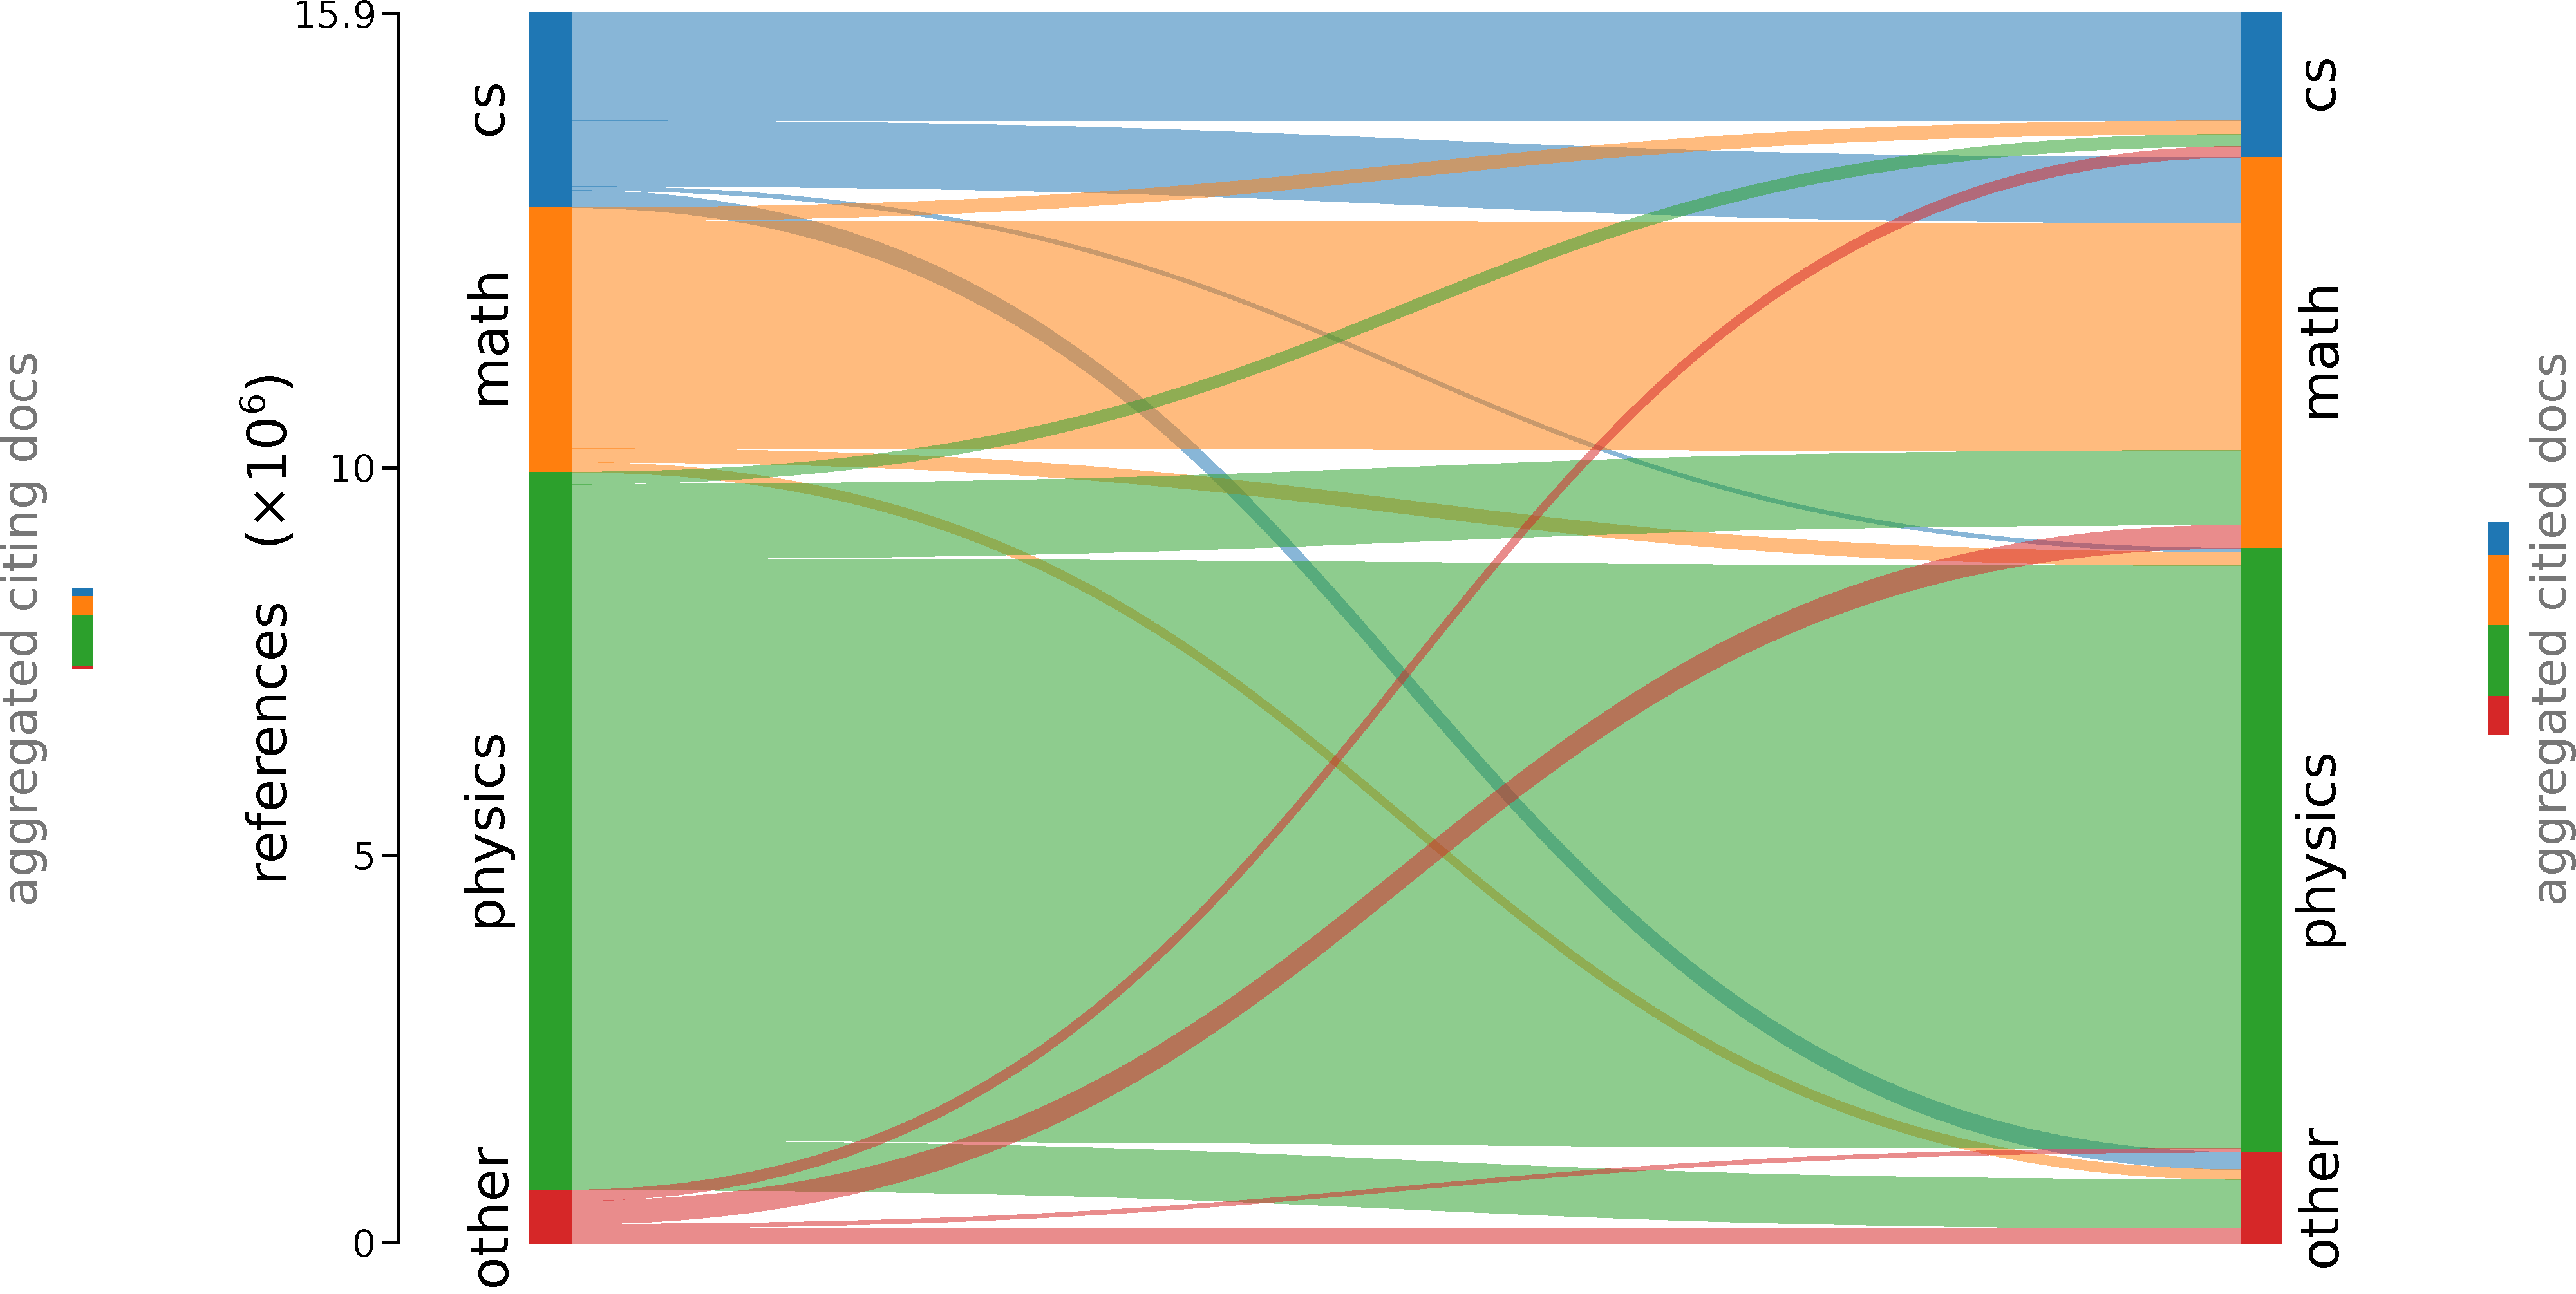
\includegraphics[width=.7\textwidth]{imgs/unarXive_citflow_sankey}
   \end{frame}

   \begin{frame}{Corpus - Conclusion}
   % \begin{columns}
   %     \column{.575\textwidth}
        \begin{itemize}
        \item \textbf{Advancements}
            \begin{itemize}
                \item More extensive
                \begin{itemize}
                    \item single domain vs multi domain
                \end{itemize}
                \item More complete, high quality citation network
                \begin{itemize}
                    \item 13.3\% increase in linked references {\color{contextgrey}($\leftrightarrow \text{S2ORC}_\text{\LaTeX}$)}
                    \item 4\% more accurate reference links {\color{contextgrey}($\leftrightarrow \text{S2ORC}_\text{\LaTeX}$)}
                \end{itemize}
                \item Less noise due to \LaTeX\ as source
                \item Novel types of analyses possible
            \end{itemize}
        \item \textbf{Foundation for further studies}
        \item $\rightarrow$ \rtmark{1\large\checkmark}
        \end{itemize}
       % \column{.475\textwidth}
       %    \centering
   % \end{columns}
   \end{frame}


\section{Citations \& Non-English}

   \begin{frame}[plain]
        \vspace{0.7cm}
        \begin{infobox-map}
        \centering
        \begin{Huge}
        \textbf{Citations \& Non-English}\\
        \end{Huge}
        \end{infobox-map}
   \end{frame}

   \begin{frame}{Citation Network - Digest}
    % - one slide for blocking & uX22 w/ improvement stats

   \begin{columns}
       \column{.475\textwidth}
        \begin{itemize}
            \item \textbf{Research Task}\\Develop a method linking references more successfully without compromising accuracy
            \item \textbf{Method}
            \begin{itemize}
                \item Use unarXive data
                \item Improved reference linking pipeline\\(parser \& target set choice, heuristics)
                \item Blocking \& matching within set of references
            \end{itemize}
            \item \textbf{Results}
            \begin{itemize}
                \item +2\% in base matching success (SOTA)
                \item Manifold increase in bibl. couplings
            \end{itemize}
            \item $\rightarrow$ \rtmark{2\large\checkmark}
        \end{itemize}
       \column{.475\textwidth}
            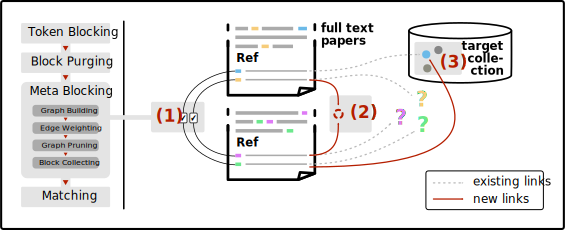
\includegraphics[width=\linewidth]{imgs/blocking_schema}
           \begin{infobox-pub-small}
           \textbf{ULITE'22}~\cite{Saier2022ULITE}
           \end{infobox-pub-small}
           \vspace{-0.5em}
           \begin{infobox-pub-small}
           \textbf{JCDL'23}~\cite{Saier2023unarXive}
           \end{infobox-pub-small}
   \end{columns}
   \end{frame}

   \begin{frame}{Non-English Documents - Digest}
    % - one slide w/ improvement stats and mby one analysis takeaway

   \begin{columns}
       \column{.575\textwidth}
        \vspace{-1cm}
        \begin{itemize}
            \item \textbf{Research Task}\\Develop an approach to include non-English publications into large-scale scholarly data
            \item \textbf{Method}
            \begin{itemize}
                \item Use unarXive data
                \item Identify cross-lingual citations by reference strings
                \item Temporal and geographic analyses
            \end{itemize}
            \item \textbf{Results}
            \begin{itemize}
                \item Reliable method for identification
                \item Largest study so far ($<$1k $\rightarrow$ $>$1M)
                \item Identification of trends and challenges
            \end{itemize}
            \item $\rightarrow$ \rtmark{3\large\checkmark}
        \end{itemize}
       \column{.375\textwidth}
            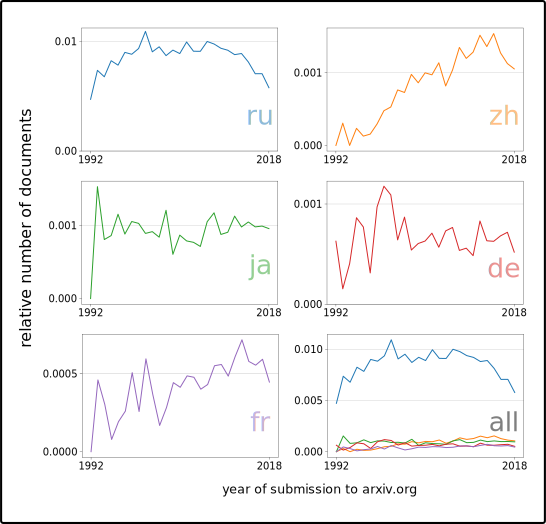
\includegraphics[width=0.8\linewidth]{imgs/xling_example_result}
           \begin{infobox-pub-small}
           \textbf{ICADL'20}~\cite{Saier2020xling}
           \end{infobox-pub-small}
           \vspace{-0.5em}
           \begin{infobox-pub-small}
           \textbf{IJDL'22}~\cite{Saier2021}
           \end{infobox-pub-small}
   \end{columns}
   \end{frame}

\section{Artifact Parameters}

   \begin{frame}[plain]
        \vspace{0.7cm}
        \begin{infobox-map}
        \centering
        \begin{Huge}
        \textbf{Artifact Parameters}\\
        \end{Huge}
        \end{infobox-map}
   \end{frame}

   \begin{frame}{Artifact Parameters}
       \begin{overprint}
           \onslide<1> \centering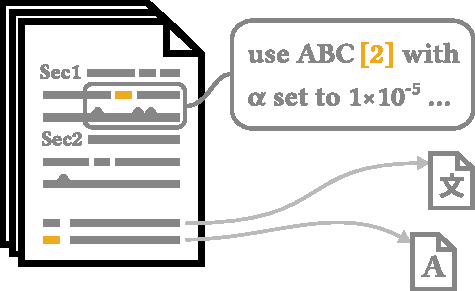
\includegraphics[width=0.4\textwidth]{imgs/schema_add_09_vargapartf_1}
           \onslide<2> \centering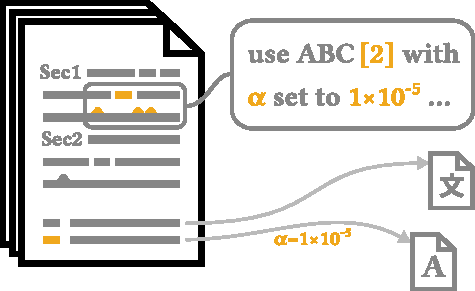
\includegraphics[width=0.4\textwidth]{imgs/schema_add_09_vargapartf_0}
       \end{overprint}
   \end{frame}

   \begin{frame}{Artifact Parameters - Motivation}
       \begin{overprint}
           \onslide<1> \centering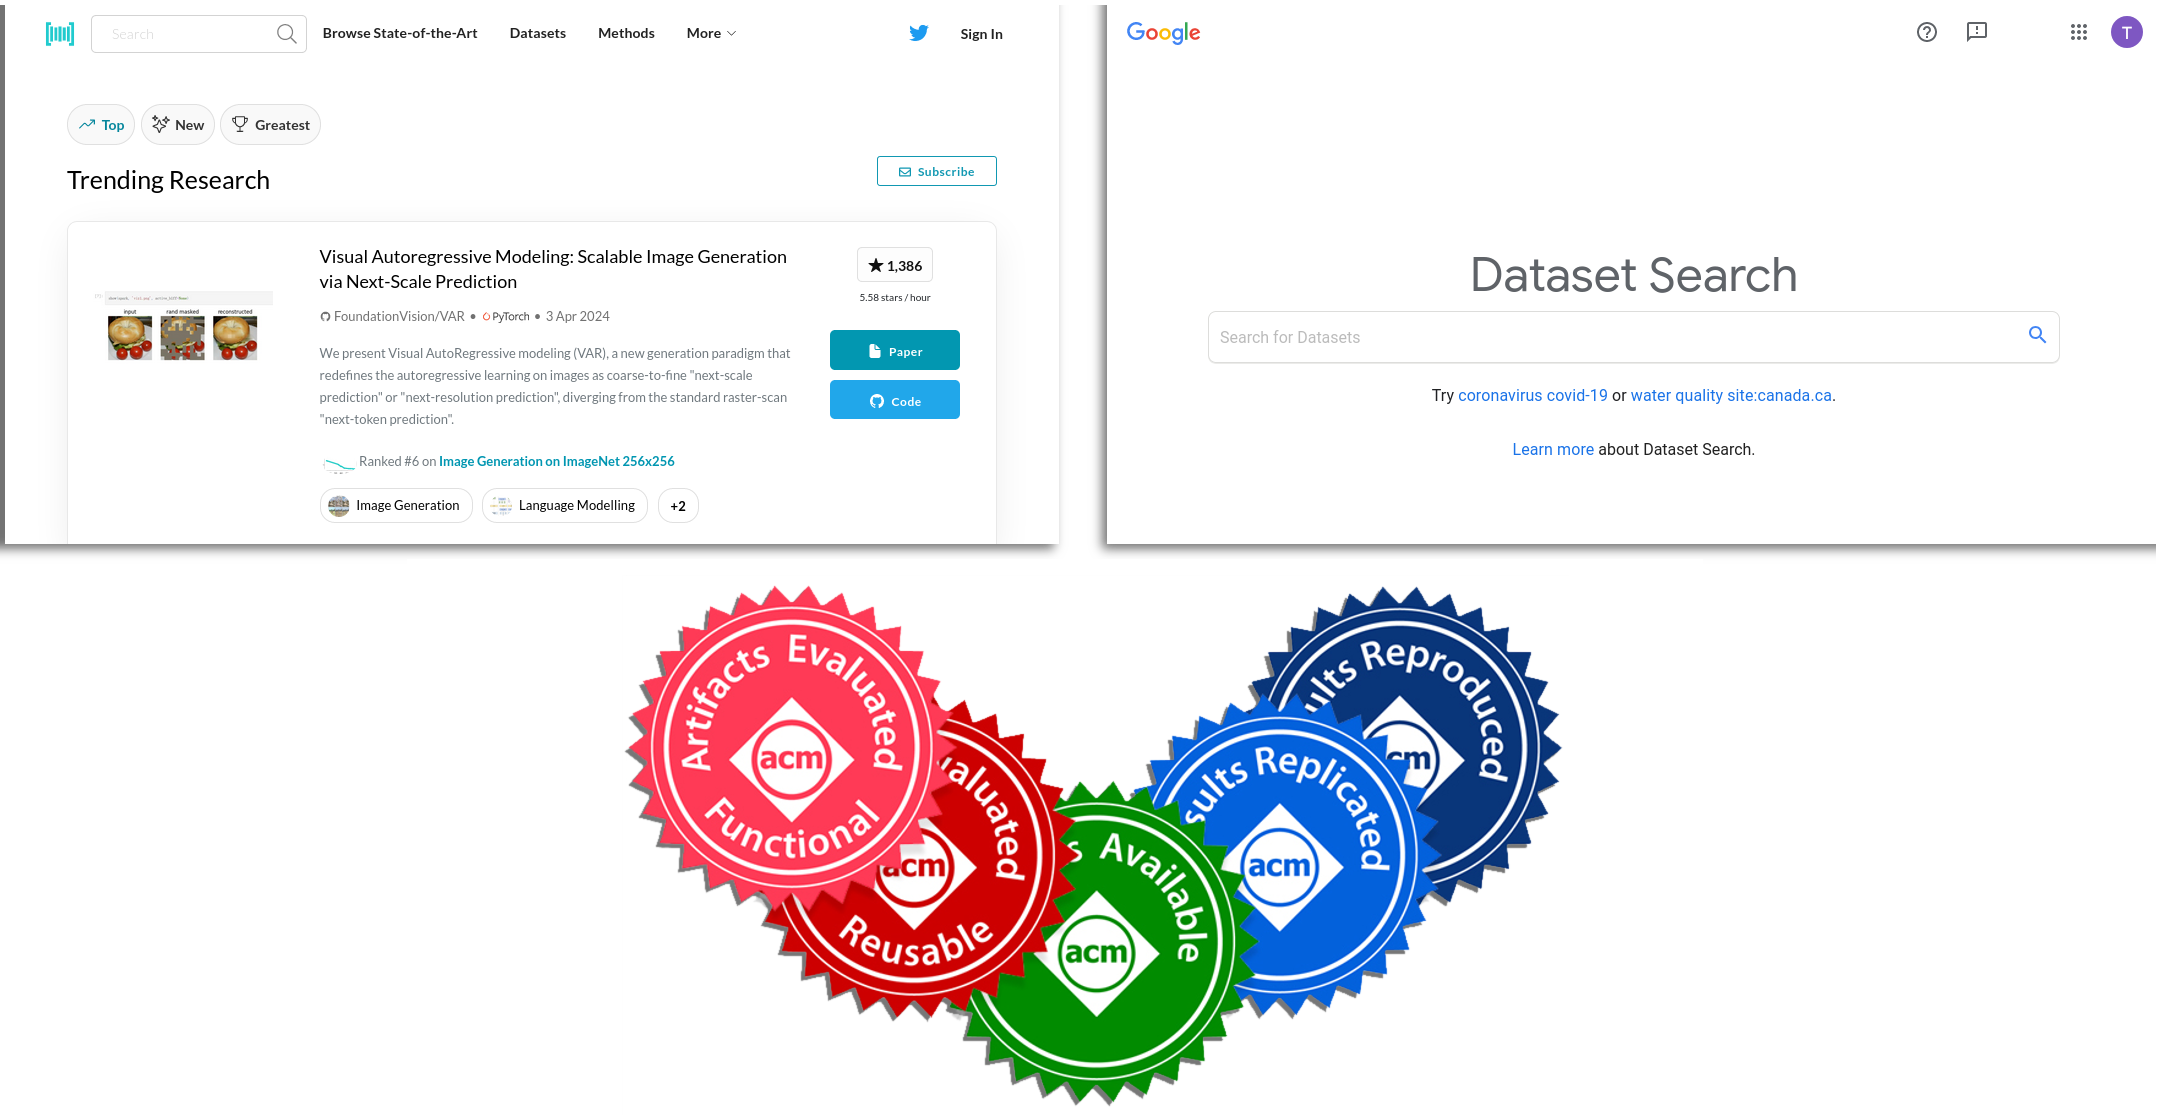
\includegraphics[width=.75\textwidth]{imgs/artifacts_en}
           \onslide<2> \centering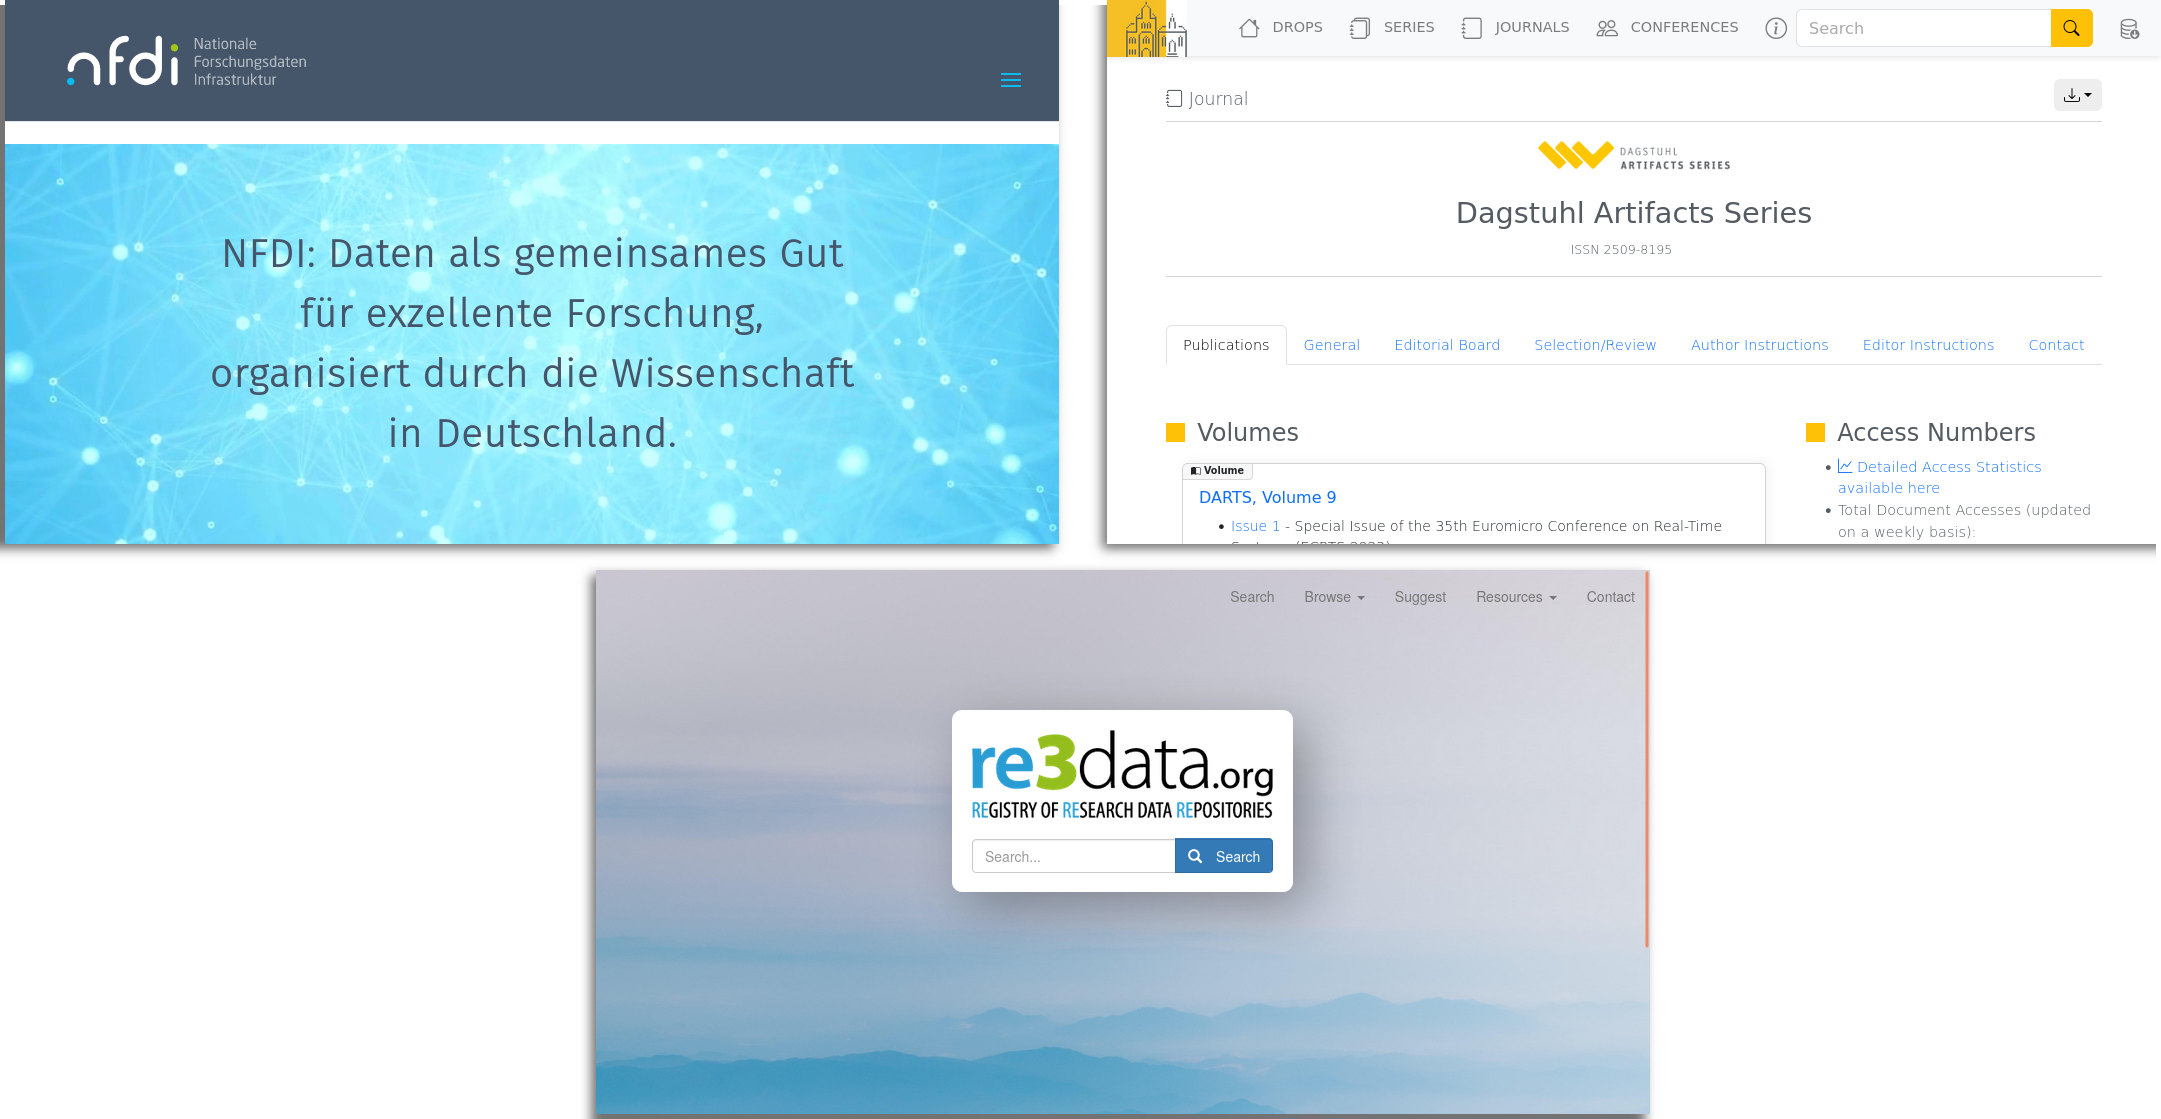
\includegraphics[width=.75\textwidth]{imgs/artifacts_de}
           \onslide<3> \centering \vspace{1.25em}\begin{large}NLP field increasing focus on \textbf{data} and its \textbf{algorithmic processing}\end{large}\\\vspace{1em}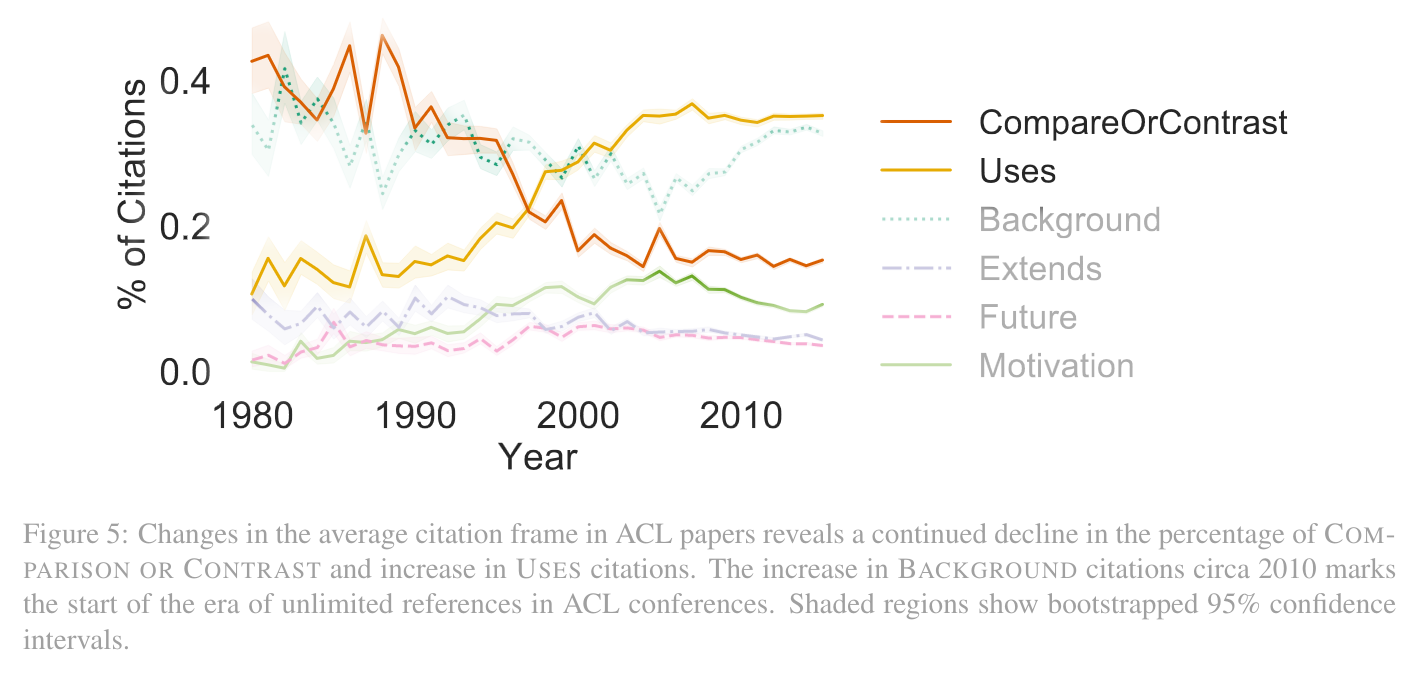
\includegraphics[width=.5\textwidth]{imgs/use_on_the_rise_e}\\\begin{tiny}\fullcite{Jurgens2018}\end{tiny}
       \end{overprint}
   \end{frame}

   \begin{frame}{Artifact Parameters - Digest}
    % - why useful, why challenging
    % - highlight trends in focussing on research artifacts
    %   - DARTS (https://www.dagstuhl.de/en/publishing/series/details/DARTS)
    %   - re3data (https://www.re3data.org/)
    %   - Papers with Code
    %   - ACM Artifact Review and Badging (https://www.acm.org/publications/policies/artifact-review-and-badging-current)

   \begin{columns}
       \column{.475\textwidth}
        \begin{itemize}
            \item \textbf{Research Task}\\Develop a method to extract fine-grained research artifacts information
            \item \textbf{Method}
            \begin{itemize}
                \item Task formalization
                \item Data annotation {\color{lightgrey}(data from unarXive)}
                \item Two lines of approaches
                \begin{itemize}
                    \item BERT based model approach
                    \item LLM based approach
                \end{itemize}
            \end{itemize}
            \item \textbf{Results}
            \begin{itemize}
                \item Novel task, novel data
                \item Improvements over SOTA baselines
                \item Methods applicable to large data sets
            \end{itemize}
        \end{itemize}
       \column{.475\textwidth}
            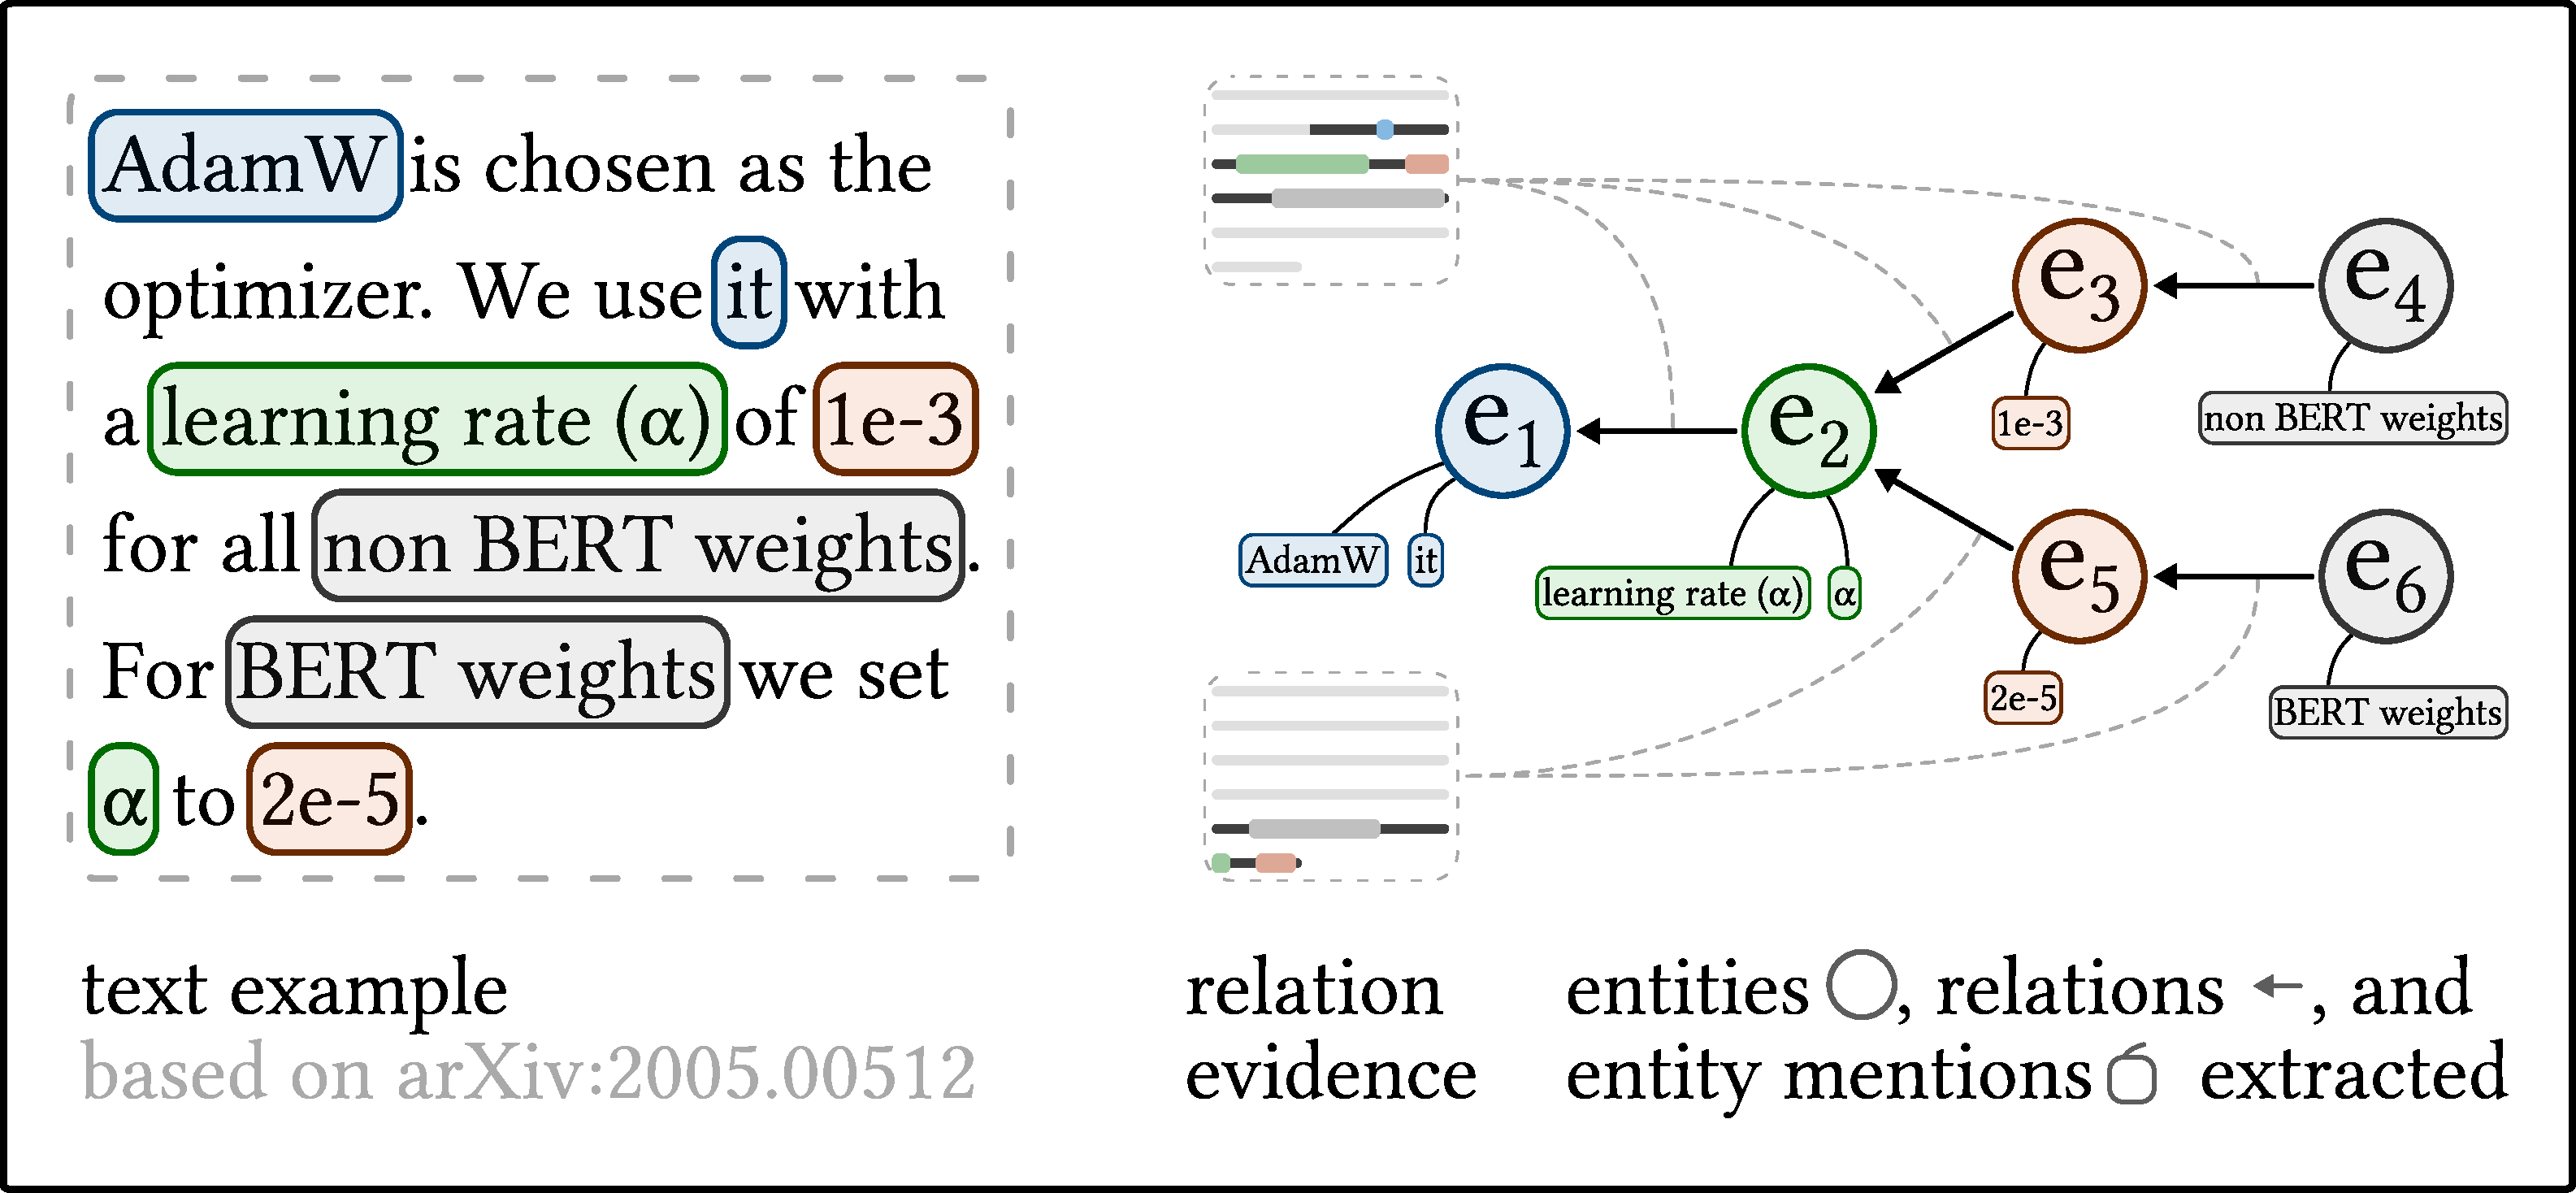
\includegraphics[width=\linewidth]{imgs/hyperpie_schema}
           \begin{infobox-pub-small}
           \textbf{ECIR'24}~\cite{Saier2024HyperPIE}
           \end{infobox-pub-small}
   \end{columns}
   \end{frame}

   %\begin{frame}{Examples}
   %\begin{itemize}
   %    \item ``For ADAM, we set $\beta_2 = 0.999$ for all our experiments''\\
   %            (\texttt{arXiv:1807.06766})
   %    % \item ``The learning rate is set to $0.001$ for LSTM and ours and $0.0001$ for C3D as the learning was unstable with bigger learning rates.''\\
   %    %         (\texttt{arXiv:1807.06980})
   %    %\item ``For Omniglot, we use train/valid/test split of $23,845/500/8,070$ images.''\\
   %    %        (\texttt{arXiv:1812.10539})
   %    \item ``We consider image resolutions of $64\times64$ and $256\times256$ on Dayton dataset while for experiments on CVUSA dataset, $256\times256$ resolution images are used.''\\
   %            (\texttt{arXiv:1803.03396})
   %\end{itemize}
   %\end{frame}

   % \begin{frame}{Artifact Parameters - Task Definition}
   % \begin{itemize}
   %     \item \textbf{Goal}
   %     \begin{itemize}
   %         \item Automatically extract parameter information from paper text
   %     \end{itemize}
   %     \item \textbf{Motivation}
   %     \begin{itemize}
   %         \item Reproducibility indication~\cite{Radd2019}, automation~\cite{sethi2018}
   %         \item Uncover conventions and trends
   %         \item More fine-grained paper representations (similarity measures, recommendation, search)
   %     \end{itemize}
   %     \item \textbf{Task Type}
   %     \begin{itemize}
   %         \item (Named) Entity Recognition, Relation Extraction \hphantom{mmmmm} \smash{\includegraphics[height=2.75\fontcharht\font`\B]{imgs/ner_el_c}}
   %     \end{itemize}
   %     % \item \textbf{Approach}
   %     % \begin{itemize}
   %     %     \item Manually annotated data set
   %     %     \item Fine-tuned models in supervised setting
   %     %     \item LLMs in zero-/few-shot setting
   %     % \end{itemize}
   % \end{itemize}
   % \end{frame}

   % \begin{frame}{Artifact Parameters - Scope \& Annotation Scheme}
   % \begin{itemize}
   %     \item 4 entity classes
   %     \begin{itemize}
   %         \item (1) research \textbf{artifact}: model, method, data set, ...
   %         \item descriptions of how authors use the artifacts\\
   %              (2) \textbf{parameter} ($\alpha$, learning rate, k, ...)\\
   %              (3) \textbf{value} (1e-3, five, $\frac{1}{3}$, ...)\\
   %              (4) \textbf{context} (for fine-tuning, during grid search, ...)
   %     \end{itemize}
   %     \item 1 relation type
   %     \item out of scope
   %         \begin{itemize}
   %              \item measurements (\textit{``We obtain an AUC value of 0.75''})
   %              % \item IE from tabes, code, etc.
   %         \end{itemize}
   % \end{itemize}
   % \end{frame}

   % \begin{frame}{Scope \& Annotation Scheme}
   %     \centering
   %     \includegraphics[width=0.75\textwidth]{imgs/schema_visual_v3}
   % \end{frame}

   \begin{frame}{Artifact Parameters - Task}
       \begin{overprint}
           \onslide<1> \centering\includegraphics[width=0.75\textwidth]{imgs/schema_visual_praes_4}
           \onslide<2> \centering\includegraphics[width=0.75\textwidth]{imgs/schema_visual_praes_3}
           \onslide<3> \centering\includegraphics[width=0.75\textwidth]{imgs/schema_visual_praes_2}
           \onslide<4> \centering\includegraphics[width=0.75\textwidth]{imgs/schema_visual_praes_1}
           \onslide<5> \centering\includegraphics[width=0.75\textwidth]{imgs/schema_visual_praes_0}
       \end{overprint}
   \end{frame}

   \begin{frame}{Artifact Parameters - Related Work: Fine-tuned models}
   \begin{columns}
       \column{.475\textwidth}
           \begin{itemize}
               \item SciERC dataset % (paragraph level)
                   \begin{itemize}
                       \item SCIIE~\cite{luan2018scierc}
                       \item PL-Marker~\cite{Ye2022}
                       \item \textbf{$\rightarrow$ entity type overlap}
                   \end{itemize}
               \item [[~~...]]
               % \item {\color{contextgrey}SciREX dataset} % (document level)
               %     \begin{itemize}
               %         {\item \color{contextgrey}TempGen~\cite{Huang2021} (only RE)}
               %     \end{itemize}
               % \item {\color{contextgrey}SemEval 2022 (math symb. to descr.)}
               %     \begin{itemize}
               %         \item {\color{contextgrey}JBNU-CCLab~\cite{Lee2022}}
               %         \item {\color{contextgrey}AIFB~\cite{Popovic2022}}
               %     \end{itemize}
               \item SemEval 2021 (measurements)
                   \begin{itemize}
                       \item LIORI~\cite{Davletov2021}
                       \item \textbf{$\rightarrow$ utilize mention pattern regularities}
                   \end{itemize}
           \end{itemize}
       \column{.475\textwidth}
           \begin{center}\includegraphics[width=\textwidth]{imgs/scirex}\end{center}
   \end{columns}
   \end{frame}

   \begin{frame}{Artifact Parameters - Related Work: LLMs}
   \begin{columns}
       \column{.475\textwidth}
           \begin{itemize}
               \item Medical science~\cite{Agrawal2022}
                   \begin{itemize}
                       \item singular values
                       \item lists
                   \end{itemize}
               \item Material science~\cite{Xie2023,Polak2023,Dunn2022}
                   \begin{itemize}
                       \item singular values
                       \item lists
                       \item hierarchical~\cite{Dunn2022} (see right)\\\textbf{$\rightarrow$ data serialization format}
                   \end{itemize}
           \end{itemize}

          ‌\\
          Note: all of the above evaluate\\
          on GPT models only.
       \column{.475\textwidth}
           \begin{center}\includegraphics[width=0.9\textwidth]{imgs/llm_sciext}\\{\tiny\fullcite{Dunn2022}\par}\end{center}
   \end{columns}
   \end{frame}

   \begin{frame}{Approach: Fine-tuned models}
   \begin{columns}
       \column{.375\textwidth}
           \begin{itemize}
               \item Based on PL-Marker\\(SciERC SOTA)
               \item (N)ER: used as is
               \item RE: new module, utilizing
               \begin{itemize}
                   \item Entity class embeddings
                   \item Entity distance
               \end{itemize}
           \end{itemize}
       \column{.575\textwidth}
           \includegraphics[width=\linewidth]{imgs/ffnn_re_sub_visual_v2}
   \end{columns}
   \end{frame}

   \begin{frame}{Approach: LLMs}
   \begin{columns}
       \column{.375\textwidth}
           \begin{itemize}
               % \item Test various prompting techniques
               % \begin{itemize}
               %     \item Multi-stage
               %     \item In-text annitation
               %     \item Data serialization format \checkmark
               % \end{itemize}
               \item Data serialization format
               \begin{itemize}
                    \item JSON $\rightarrow$ YAML
               \end{itemize}
               \item Compare 6 models
               \item Base prompt + tuning for each
               \item Zero-shot: all
               \item Few-shot: only Vicuna${}_\text{16k}$
               % \begin{itemize}
               %     \item gBNF grammar
               % \end{itemize}
           \end{itemize}
       \column{.575\textwidth}
        \begin{overlayarea}{\textwidth}{2.45cm}
        \only<1>{
           \includegraphics[width=\linewidth]{imgs/llm_nerre_visual_v2}
        }
        \only<2>{
        \begin{table}
        \centering
          % \caption[LLM selection]{LLM selection (size in number of parameters).}
          % \label{tab:llmselection}
          \begin{tabular}{llc}
            \hline
            Model & Size \\ % & Variant
            \hline
            WizardLM~\cite{xu2023wizardlm2023}
            %& \texttt{WizardLM-13B-V1.1}
            & 13\,B \\
            Vicuna${}_{4k}$~\cite{vicuna2023}
            %& \texttt{vicuna-13b-v1.3}
            & 13\,B \\
            Vicuna${}_{16k}$~\cite{vicuna2023}
            %& \texttt{vicuna-13b-v1.5-16k}
            & 13\,B \\
            Falcon~\cite{falcon40b-huggingface}
            %& \texttt{falcon-40b-instruct}
            & 40\,B \\
            GALACTICA~\cite{GALACTICA2022}
            %& \texttt{galactica-120b}
            & 120\,B \\
            GPT-3.5~\cite{Brown2020gpt3}
            %& \texttt{text-davinci-003}
            & 175\,B \\
            \hline
            \end{tabular}
        \end{table}
        }
        \end{overlayarea}
   \end{columns}
   \end{frame}

   \begin{frame}{Artifact Parameters - Data}
   \begin{columns}
       \column{.375\textwidth}
           \begin{itemize}
               \item No existing data sets\\$\rightarrow$ use unarXive ML/CV/CL/DL
               \item Annotation approach
               \begin{itemize}
                  %\item Guidelines based on ACL RD-TEC guidelines~\cite{Qasemizadeh2016}
                  \item Paragraph level, whole papers
               \end{itemize}
               \item Extent
               \begin{itemize}
                  \item 444 paragraphs
                  \item 1,971 entities\\(1,134 a, 131 p, 662 v, 44 c)
                  \item 614 relations
               \end{itemize}
               \item IAA
               \begin{itemize}
                  \item 0.867 for entities
                  \item 0.737 for relations
               \end{itemize}
           \end{itemize}
       \column{.575\textwidth}
        \only<1>{
            \centering
            \includegraphics[width=.8\linewidth]{imgs/annot_guidelines}
        }
        % \only<2>{
        %     \begin{figure}
        %         \centering
        %         \subfloat[text segments\label{fig:text-seg-size}]{%
        %             \includegraphics[width=.35\linewidth]{imgs/text_span_size_stats}
        %         }
        %         \subfloat[relation distances (\#chars)\label{fig:rel-dists}]{%
        %             \includegraphics[width=.53\linewidth]{imgs/stats_artifact_param_value_distance-crop}
        %         }
        %         \caption{Observations of initial annotation round}
        %         \label{fig:init-annot}
        %     \end{figure}
        % }
   \end{columns}
   \end{frame}

   \begin{frame}{Artifact Parameters - Experiments: Fine-tuned models}
   \begin{columns}
       \column{.375\textwidth}
           \begin{itemize}
               \item \textbf{Setting}
               \begin{itemize}
                   \item 5-fold cross-validation
                   \item Stratified sampling
               \end{itemize}
               \item \textbf{Results} ($\text{F}_1$\,[\%])
               \begin{itemize}
                  \item ER: 78.0
                  \item RE: 9.9 $\rightarrow$ 38.8
               \end{itemize}
               \item \textbf{Analysis}
               \begin{itemize}
                  \item Parameter: low performance
                  \item Contexts: not predicted
               \end{itemize}
           \end{itemize}
       \column{.575\textwidth}
        \begin{overlayarea}{\textwidth}{3cm}
        \only<2>{
           \includegraphics[width=\linewidth]{imgs/fine_tuned_eval}
        }
        \only<3>{
        \begin{table}
          \centering
          \caption[Ablation study results]{Ablation study results (model inputs are: T = BERT token embeddings, C = entity class embeddings, D = entity distance)}
          \label{tab:finetunedablation}
          \begin{tabular}{lccc}
            \hline
            Used & P [\%] & R [\%] & $\text{F}_1$\,[\%] \\
            \hline
            \textvisiblespace CD & 15.5 & 8.8 & 11.1 \\
            T\textvisiblespace D & 16.6 & 29.8 & 19.6 \\
            TC\textvisiblespace & 26.5 & 65.0 & 35.5 \\
            TCD & \textbf{30.7} & \textbf{65.0} & \textbf{38.8} \\
            \hline
          \end{tabular}
        \end{table}
        }
        \end{overlayarea}
   \end{columns}
   \end{frame}


   % \begin{frame}{Artifact Parameters - Experiments: LLMs}
   %  \begin{table}
   %    \begin{center}
   %    \label{tab:llmeval}
   %    \begin{tabular}{ll|ccc|ccc}
   %      \hline
   %      \ & \ & \multicolumn{3}{c|}{Entity Recognition}
   %        & \multicolumn{3}{c}{Relation Extraction} \\
   %      \hline
   %      Model & Output & P [\%] & R [\%] & $\text{F}_1$ [\%] &
   %                       P [\%] & R [\%] & $\text{F}_1$ [\%] \\
   %      \hline
   %      \multirow{2}{*}{Falcon} &
   %      JSON & \textbf{35.9} & 5.9 & 10.2
   %                & 0.0 & 0.0 & 0.0 \\
   %      \ & YAML & 26.3 & 14.3 &
   %      \hphantom{${}_{\Delta\text{+8.3}}$}
   %      18.5{\color{parametergreen}{${}_{\Delta\text{+8.3}}$}}
   %                & 0.0 & 0.0 &
   %      \hphantom{${}_{\Delta\text{+0.0}}$}
   %      0.0{\color{contextgrey}{${}_{\Delta\text{+0.0}}$}}  \\
   %      \multirow{2}{*}{GALACTICA} &
   %      JSON & 25.9 & 15.7 & 19.5
   %                & 0.1 & 2.3 & 0.3 \\
   %      \ & YAML & 20.9 & 19.3 &
   %      \hphantom{${}_{\Delta\text{+0.6}}$}
   %      20.1{\color{parametergreen}{${}_{\Delta\text{+0.6}}$}}
   %                & 0.0 & 0.8 &
   %      \hphantom{${}_{\Delta\text{-0.2}}$}
   %      0.1{\color{valuered}{${}_{\Delta\text{-0.2}}$}}  \\
   %      \multirow{2}{*}{WizardLM} &
   %      JSON & 6.8 & 11.3 & 8.5
   %                & 0.1 & 0.8 & 0.1 \\
   %      \ & YAML & 11.3 & 33.7 &
   %      \hphantom{${}_{\Delta\text{+8.5}}$}
   %      17.0{\color{parametergreen}{${}_{\Delta\text{+8.5}}$}}
   %                & 0.2 & 3.8 &
   %      \hphantom{${}_{\Delta\text{+0.3}}$}
   %      0.4{\color{parametergreen}{${}_{\Delta\text{+0.3}}$}}  \\
   %      \multirow{2}{*}{Vicuna} &
   %      JSON & 13.4 & 9.3 & 11.0
   %                & 0.7 & 3.8 & 1.1 \\
   %      \ & YAML & 15.5 & 41.6 &
   %      \hphantom{${}_{\Delta\text{+11.6}}$}
   %      22.6{\color{parametergreen}{${}_{\Delta\text{+11.6}}$}}
   %                & 0.2 & 3.8 &
   %      \hphantom{${}_{\Delta\text{-0.6}}$}
   %      0.5{\color{valuered}{${}_{\Delta\text{-0.6}}$}}  \\
   %      \multirow{2}{*}{GPT-3.5} &
   %      JSON & 27.9 & \textbf{42.8} & \underline{33.8}
   %                & \underline{5.4} & \underline{10.7} & \underline{7.2} \\
   %      \ & YAML & \underline{33.9} & \underline{41.7} &
   %      \hphantom{${}_{\Delta\text{+3.6}}$}
   %      \textbf{37.4}{\color{parametergreen}{${}_{\Delta\text{+3.6}}$}}
   %                & \textbf{5.8} & \textbf{12.2} &
   %      \hphantom{${}_{\Delta\text{+0.6}}$}
   %      \textbf{7.8}{\color{parametergreen}{${}_{\Delta\text{+0.6}}$}}  \\
   %    \hline
   %    \end{tabular}
   %    \end{center}
   %  \end{table}
   % \end{frame}


   \begin{frame}{Artifact Parameters - Experiments: LLMs}
   \begin{columns}
       \column{.375\textwidth}
           \vspace{-4em}
           \begin{itemize}
               \item \textbf{Setting}
               \begin{itemize}
                   \item Zero-/5-shot
                   \item Compare JSON w/ YAML variant
               \end{itemize}
               \item \textbf{Results} (best ER / RE $\text{F}_1$\,[\%])
               \begin{itemize}
                  \item Zero-shot: 37.4 / 7.8
                  \item 5-shot: 44.0 / 6.1
               \end{itemize}
               \item \textbf{Analysis}
               \begin{itemize}
                  \item Very low RE performance
                  \item YAML: avg. +5\% in ER
                  \item 5-shot: +27\% ER, +6\% RE
                  \item Format adherence\\+ entity hallucinations
               \end{itemize}
           \end{itemize}
       \column{.575\textwidth}
        \begin{overlayarea}{\textwidth}{7cm}
        \only<2>{

    \begin{table}
     \begin{small}
      \centering
      %\caption[Prediction performance of LLM models]{Prediction performance of LLM models. Subscripts (${}_{\Delta\pm n}$) show the delta in $\text{F}_1$ from JSON to YAML output of each model. Format: \textbf{best}, \underline{second}.}
      \begin{tabular}{ll|cc}
        \hline
        \multicolumn{2}{l|}{\textbf{Zero-shot}} &
        ER &
        RE \\
        \hline
        Model & Output & $\text{F}_1$\,[\%] &
                         $\text{F}_1$\,[\%] \\
        \hline

        \multirow{2}{*}{WizardLM} &
        JSON & 8.6
             &  0.1 \\
        \ & YAML &
        \hphantom{${}_{\Delta\text{+6.7}}$}
        15.3{\color{parametergreen}{${}_{\Delta\text{+6.7}}$}}
                  &
        \hphantom{${}_{\Delta\text{+0.0}}$}
        0.1{\color{contextgrey}{${}_{\Delta\text{+0.0}}$}}  \\
        \cline{1-2}

        \multirow{2}{*}{Vicuna${}_{4k}$} &
        JSON & 11.5
             & 1.2 \\
        \ & YAML &
        \hphantom{${}_{\Delta\text{+10.8}}$}
        22.3{\color{parametergreen}{${}_{\Delta\text{+10.8}}$}}
                  &
        \hphantom{${}_{\Delta\text{-1.1}}$}
        0.1{\color{valuered}{${}_{\Delta\text{-1.1}}$}}  \\
        \cline{1-2}

        \multirow{2}{*}{Falcon} &
        JSON & 10.2
             & 0.0 \\
        \ & YAML &
        \hphantom{${}_{\Delta\text{+9.6}}$}
        19.8{\color{parametergreen}{${}_{\Delta\text{+9.6}}$}}
                  &
        \hphantom{${}_{\Delta\text{+0.0}}$}
        0.0{\color{contextgrey}{${}_{\Delta\text{+0.0}}$}}  \\
        \cline{1-2}

        \multirow{2}{*}{GALACTICA} &
        JSON & 19.5
             & 0.3 \\
        \ & YAML &
        \hphantom{${}_{\Delta\text{+1.6}}$}
        21.1{\color{parametergreen}{${}_{\Delta\text{+1.6}}$}}
                  &
        \hphantom{${}_{\Delta\text{-0.2}}$}
        0.1{\color{valuered}{${}_{\Delta\text{-0.2}}$}}  \\
        \cline{1-2}

        \multirow{2}{*}{GPT-3.5} &
        JSON & \underline{33.8}
             & \underline{7.2} \\
        \ & YAML &
        \hphantom{${}_{\Delta\text{+3.6}}$}
        \textbf{37.4}{\color{parametergreen}{${}_{\Delta\text{+3.6}}$}}
                  &
        \hphantom{${}_{\Delta\text{+0.6}}$}
        \textbf{7.8}{\color{parametergreen}{${}_{\Delta\text{+0.6}}$}}  \\

      \hline
        \multicolumn{2}{l|}{\textbf{5-shot}} &
        ER &
        RE \\
      \hline

        \multirow{2}{*}{Vicuna${}_{16k}$} &
        JSON & \underline{39.6}
             & \underline{1.3} \\
        \ & YAML &
        \hphantom{${}_{\Delta\text{+0.4}}$}
        \textbf{44.0}{\color{parametergreen}{${}_{\Delta\text{+0.4}}$}}
                  &
        \hphantom{${}_{\Delta\text{+4.8}}$}
        \textbf{6.1}{\color{parametergreen}{${}_{\Delta\text{+4.8}}$}}  \\
      \hline
      \end{tabular}
     \end{small}
    \end{table}

        }
        \end{overlayarea}
   \end{columns}

   \end{frame}

   \begin{frame}{Artifact Parameters - Experiments: Application}
   \begin{columns}
       \column{.575\textwidth}
        \vspace{-1.5em}
        \begin{itemize}
        \item Apply best model (BERT based) on 15k paper sample
        \item Parameters information given in
        \begin{itemize}
            \item 36\% of ML papers
            \item 42\% of CV papers
            \item 36\% of CL papers
            \item 7\% of DL papers
        \end{itemize}
        \item Distribution towards second half of paper across disciplines
        \end{itemize}
       \column{.375\textwidth}
          \centering
           \includegraphics[width=0.75\textwidth]{imgs/hyperparam_pos}
   \end{columns}
   \end{frame}

   \begin{frame}{Artifact Parameters - Conclusion}
   % - summary of results & contributions
   % \begin{columns}
   %     \column{.575\textwidth}
    \begin{itemize}
        \item \textbf{Advancements}
        \begin{itemize}
            \item Novel, relevant task\\
                  (data scheme, annotation guidelines)
            \item High quality manually annotated data set
            \item Approaches based on BERT, LLMs
                \begin{itemize}
                \item BERT model based approach\\
                      29\% F${}_1$ increase for RE
                \item LLM approach\\
                      Avg. 5.5\% F${}_1$ increase for ER\\
                      (consistent across all used LLMs)
                \end{itemize}
            \item Trained model applicable on large scale
        \end{itemize}
        \item $\rightarrow$ \rtmark{4\large\checkmark}
    \end{itemize}
       % \column{.475\textwidth}
       %    \centering
   % \end{columns}
   \end{frame}

\section{Conclusion}

   \begin{frame}[plain]
        \vspace{0.7cm}
        \begin{infobox-map}
        \centering
        \begin{Huge}
        \textbf{Conclusion}\\
        \end{Huge}
        \end{infobox-map}
   \end{frame}

   \begin{frame}[t]{Overall Conclusion}

   \begin{infobox-objective}
   \large\textbf{Research Objective}\\Develop methods for generating large-scale, high quality scholarly data.
   \end{infobox-objective}

   \vspace{.5em}
   \only<2>{
    % \rtmark{1\large\checkmark}
    % \textbf{{\color{objblue-box}\faCrosshairs}\,Research Objective \large\checkmark}
   \large
   \begin{itemize}
      \item[\rtmark{1}] Corpus Creation
      \item Citation Network
      \item Non-English Publications
      \item Research Artifacts
   \end{itemize}
   }

    % \only<2>{
    % \centering
    % \Large like this:

    % \vspace{0.3cm}
    % \includegraphics[width=0.47\linewidth]{imgs/contrib_overview_dis_var}
    % }

    % \only<3>{
    %  \begin{itemize}
    %      \item Scholarly data from source formats
    %      \item Joint handling of docs \& references
    %      \item Identifier aware references parsing
    %      \item Intra references clustering \& matching
    %      \item Extraction of non-English content
    %      \item Identification of cross-lingual references from raw references
    %      \item Extraction of usage parameters from full text
    %      \item Mention pattern aware relation extraction
    %  \end{itemize}
    %  }

   \end{frame}


   \begin{frame}[plain]
       \begin{overprint}
           \onslide<1> \centering\includegraphics[width=\textwidth]{imgs/objective_grid_and_contrib_6}
           \onslide<2> \centering\includegraphics[width=\textwidth]{imgs/objective_grid_and_contrib_conclusion_rts}
           \onslide<3> \centering\includegraphics[width=\textwidth]{imgs/objective_grid_and_contrib_conclusion_dq}
       \end{overprint}
   \end{frame}

   \begin{frame}{Overall Conclusion}
   % - summary of overall contributions
   % - overview of how work has already permeated into research community
   % - reference quality aspects & RQ
   % - ...

   \begin{columns}
       \column{.4\textwidth}
        \begin{itemize}
            \item \textbf{Research Tasks}
            \begin{itemize}
                \item Basis for research
                \begin{itemize}
                    \item Corpus creation method
                \end{itemize}
                \item Advances in three focus areas
                \begin{itemize}
                    \item Citation Network
                    \item Non-English Documents
                    \item Artifact Parameters
                \end{itemize}
            \end{itemize}
            \item \textbf{Improved}
            \begin{itemize}
                \item Completeness
                \item Accuracy
                \item Relevance
                \item Comparability
                \item Timeliness
            \end{itemize}
            \item \textbf{Impact on research community}
        \end{itemize}
       \column{.6\textwidth}
            \includegraphics[width=\linewidth]{imgs/objective_grid_and_contrib_conclusion_rts}
   \end{columns}
   \end{frame}

   \begin{frame}{Impact}
   \begin{columns}
       \column{.45\textwidth}
        Adoption by the research community.

        \begin{itemize}
            \item \textbf{Methodology}
            \begin{itemize}
                \item Document Parsing Methodology~\cite{Lo2020}
            \end{itemize}
            \item \textbf{Model dev/eval}
            \begin{itemize}
                \item Citation Recommendation~\cite{Citcom2021}~(\cite{Saier2019,HybridCite2020})
                \item Citation Analysis~\cite{Veneri2022,Xue2021}~(\cite{Saier2020xling,Saier2021})
                \item Document Retrieval~\cite{Parisot2022}
                \item Researcher Profile Embeddings~\cite{Mochihashi2023}
                \item Reference Linking~(\cite{Saier2022ULITE})
            \end{itemize}
            \item \textbf{Dataset extension}
            \begin{itemize}
                \item Link Prediction~(\cite{Saier2023cocon})
                \item NER+RE~(\cite{Saier2024HyperPIE})
            \end{itemize}
        \end{itemize}
       \column{.5\textwidth}
            \centering
            \includegraphics[width=0.75\linewidth]{imgs/a2ifork}
   \end{columns}
   \end{frame}

   \begin{frame}[plain]
        \centering

        \vspace{0.7cm}
        \begin{Huge}
        \textbf{Thank You \faSmileO}\\
        \end{Huge}

        \vspace{0.7cm}
        \begin{Large}
        \textbf{Questions?}\\
        \end{Large}
   \end{frame}

   \begin{frame}[allowframebreaks]{References}
   \footnotesize
   \printbibliography
   \end{frame}

   \appendix

   \begin{frame}[plain]
        \vspace{0.7cm}
        \begin{infobox-map}
        \centering
        \begin{Huge}
        \textbf{Extra Slides}\\
        \end{Huge}
        \end{infobox-map}
   \end{frame}

   \begin{frame}
       \frametitle<1>{Quality Dimensions}
       \frametitle<2-3>{Quality Dimensions: Completeness}
       \frametitle<4-5>{Quality Dimensions: Accuracy}
       \frametitle<6-7>{Quality Dimensions: Relevance}
       \frametitle<8-9>{Quality Dimensions: Comparability}
       \frametitle<10-12>{Quality Dimensions: Timeliness}
       \begin{overprint}
           \onslide<1> \centering\includegraphics[width=0.4\textwidth]{imgs/schema_asp_x_x}
           \onslide<2> \centering\includegraphics[width=0.4\textwidth]{imgs/schema_asp_0_0}
           \onslide<3> \centering\includegraphics[width=0.4\textwidth]{imgs/schema_asp_0_1}
           \onslide<4> \centering\includegraphics[width=0.4\textwidth]{imgs/schema_asp_1_0}
           \onslide<5> \centering\includegraphics[width=0.4\textwidth]{imgs/schema_asp_1_1}
           \onslide<6> \centering\includegraphics[width=0.4\textwidth]{imgs/schema_asp_2_0}
           \onslide<7> \centering\includegraphics[width=0.4\textwidth]{imgs/schema_asp_2_1}
           \onslide<8> \centering\includegraphics[width=0.4\textwidth]{imgs/schema_asp_3_0}
           \onslide<9> \centering\includegraphics[width=0.4\textwidth]{imgs/schema_asp_3_1}
           \onslide<10> \centering\includegraphics[width=0.4\textwidth]{imgs/schema_asp_4_0}
           \onslide<11> \centering\includegraphics[width=0.4\textwidth]{imgs/schema_asp_4_1}
           \onslide<12> \centering\includegraphics[width=0.4\textwidth]{imgs/schema_asp_4_2}
       \end{overprint}
   \end{frame}

   \begin{frame}{Corpus - Stats}
    \begin{table}
    \centering
      % \caption{Overview of the proposed data set}
      % \label{tbl:allthestats}
    \begin{small}
    \begin{tabular}{lrcc|cc}
    \toprule
        \ & \ & citing & \ & \ & cited \\
        \ & \ & documents & \multicolumn{2}{c}{references} & documents \\
        \ & \ & \  & \tiny{outgoing} & \tiny{incoming} & \  \\
        \emph{full data set:} & \ & \textbf{1,043,126} & 15,954,664 & 15,954,664 & \textbf{2,746,288} \\
        &\tiny{full text}&\tiny{1,043,126}&\tiny{15,954,664}&\tiny{7,181,576}&\tiny{736,597}\\
        &\tiny{linked to MAG}&\tiny{994,351}&\tiny{15,846,351}&\tiny{15,954,664}&\tiny{2,746,288}\\
        \emph{by discipline:} & \ & \ & \ & \ & \ \\
        \multicolumn{2}{r}{physics} & 662,894 & 9,300,576 & 7,827,072 & 921,852 \\
        \multicolumn{2}{r}{mathematics} & 237,422 & 3,426,117 & 5,062,033 & 906,301 \\
        \multicolumn{2}{r}{computer science} & 111,694 & 2,526,656 & 1,876,401 & 425,860 \\
        \multicolumn{2}{r}{other} & 31,116 & 701,315 & 1,189,158 & 492,275 \\
      \bottomrule
        \\
        \multicolumn{6}{l}{
            \begin{tabular}{rl}
                \textbf{data}: & \url{http://doi.org/10.5281/zenodo.3385851} \\
                \textbf{code}: & \url{https://github.com/IllDepence/unarXive} \\
            \end{tabular}
            }
    \end{tabular}
    \end{small}
    \end{table}
   \end{frame}

   \begin{frame}{Corpus - Citation Flow}
    \centering
    \includegraphics[width=.7\textwidth]{imgs/unarXive_citflow}
   \end{frame}

   \begin{frame}{Corpus - Reference Composition}
    \centering
    \includegraphics[width=.7\textwidth]{imgs/unarXive_refcompo}
   \end{frame}

   \begin{frame}{Corpus - Target Sec. Specific Refs}
    \begin{table}
    \centering
    \begin{scriptsize}
     \begin{threeparttable}
    \begin{tabular}{llrrr}
    \toprule
       \ & Discipline\tnote{a} & Count & Normalization factor & Normalized ratio (\%) \\ % "normalized count"
       \midrule
       \textbf{Citing} & Mathematics & 298,009 & 4.66 & 8.70 \\ % 1,388,722
       \ & CS & 9,123 & 6.31 & 0.36 \\ % 57,608
       \ & Physics & 30,593 & 1.72 & 0.33 \\ % 52,480
       \midrule
       \textbf{Cited} & Mathematics & 313,651 & 3.15 & 6.20 \\ % 988,574
       \ & CS & 12,179 & 8.50 & 0.65 \\ % 103,556
       \ & Physics & 31,087 & 2.04 & 0.40 \\ % 63,368
       \midrule
       \textbf{Pairs} & \underline{Math\textsuperscript{\textdagger}$\rightarrow$Math\textsuperscript{\textdaggerdbl}} & 200,859 & 5.41 & 6.81 \\ % 1,087,290
       \ & Math\textsuperscript{\textdagger}$\rightarrow$CS & 5,134 & 92.13 & 2.96 \\ % 472,995
       \ & Math\textsuperscript{\textdagger}$\rightarrow$Phys & 3,114 & 89.88 & 1.75 \\ % 279,900
       \ & CS$\rightarrow$Math\textsuperscript{\textdaggerdbl} & 3,456 & 18.82 & 0.41 \\ % 65,028
       \ & Phys$\rightarrow$Math\textsuperscript{\textdaggerdbl} & 3,859 & 16.49 & 0.40 \\ % 63,653
       \ & \underline{CS$\rightarrow$CS} & 2,500 & 11.38 & 0.18 \\ % 28,448
       \ & \underline{Phys$\rightarrow$Phys} & 10,374 & 2.12 & 0.14 \\ % 21,941
       \ & CS$\rightarrow$Phys & 50 & 307.16 & 0.10 \\ % 15,358
       \ & Phys$\rightarrow$CS & 137 & 101.40 & 0.09  \\ % 13,892
      \bottomrule
    \end{tabular}
     \begin{tablenotes}
        \item[a] {\color{contextgrey}\textsuperscript{\textdagger}:~Mathematics citing document, \textsuperscript{\textdaggerdbl}:~Mathematics cited document, \underline{X$\rightarrow$X}:~Citing and cited document are from the same discipline.}
      \end{tablenotes}
     \end{threeparttable}
    \end{scriptsize}
    \end{table}
   \end{frame}

   \begin{frame}{Artifact Parameters - Task}
   \begin{itemize}
       \item \textbf{Task Type}
       \begin{itemize}
           \item (Named) Entity Recognition, Relation Extraction
       \end{itemize}
       \item 4 entity classes
       \begin{itemize}
           \item (1) research \textbf{artifact}: model, method, data set, ...
           \item descriptions of how authors use the artifacts\\
                (2) \textbf{parameter} ($\alpha$, learning rate, k, ...)\\
                (3) \textbf{value} (1e-3, five, $\frac{1}{3}$, ...)\\
                (4) \textbf{context} (for fine-tuning, during grid search, ...)
       \end{itemize}
       \item 1 relation type
       \begin{itemize}
           \item Given by entity type pair
       \end{itemize}
       % \item out of scope
       %     \begin{itemize}
       %          \item measurements (\textit{``We obtain an AUC value of 0.75''})
       %          % \item IE from tabes, code, etc.
       %     \end{itemize}
       % \item \textbf{Approach}
       % \begin{itemize}
       %     \item Manually annotated data set
       %     \item Fine-tuned models in supervised setting
       %     \item LLMs in zero-/few-shot setting
       % \end{itemize}
   \end{itemize}
   \end{frame}

   \begin{frame}{Artifact Parameters - Task (ext)}
   \begin{itemize}
       \item \textbf{Goal}
       \begin{itemize}
           \item Automatically extract hyperparameter information from paper text
       \end{itemize}
       \item \textbf{Motivation}
       \begin{itemize}
           \item Reproducibility indication~\cite{Radd2019}, automated reproduction~\cite{sethi2018}
           \item Uncover conventions and trends
           \item More fine-grained paper representations (similarity measures, recommendation, search)
       \end{itemize}
       \item \textbf{Task Type}
       \begin{itemize}
           \item (Named) Entity Recognition, Relation Extraction %\hphantom{mmmmm} \smash{\includegraphics[height=2.75\fontcharht\font`\B]{imgs/ner_el_c}}
       \end{itemize}
       % \item \textbf{Approach}
       % \begin{itemize}
       %     \item Manually annotated data set
       %     \item Fine-tuned models in supervised setting
       %     \item LLMs in zero-/few-shot setting
       % \end{itemize}
   \end{itemize}
   \end{frame}

   \begin{frame}{Artifact Parameters - Related Work: Fine-tuned models}
   \begin{columns}
       \column{.475\textwidth}
           \begin{itemize}
               \item SciERC dataset % (paragraph level)
                   \begin{itemize}
                       \item SCIIE~\cite{luan2018scierc}
                       \item PL-Marker~\cite{Ye2022}
                       \item \textbf{$\rightarrow$ entity type overlap}
                   \end{itemize}
               \item {\color{contextgrey}SciREX dataset} % (document level)
                   \begin{itemize}
                       {\item \color{contextgrey}TempGen~\cite{Huang2021} (only RE)}
                   \end{itemize}
               \item {\color{contextgrey}SemEval 2022 (math symb. to descr.)}
                   \begin{itemize}
                       \item {\color{contextgrey}JBNU-CCLab~\cite{Lee2022}}
                       \item {\color{contextgrey}AIFB~\cite{Popovic2022}}
                   \end{itemize}
               \item SemEval 2021 (measurements)
                   \begin{itemize}
                       \item LIORI~\cite{Davletov2021}
                       \item \textbf{$\rightarrow$ utilize mention pattern regularities}
                   \end{itemize}
           \end{itemize}
       \column{.475\textwidth}
           \begin{center}\includegraphics[width=\textwidth]{imgs/scirex}\end{center}
   \end{columns}
   \end{frame}

   \begin{frame}{Artifact Parameters - Related Work: Fine-tuned models (other data sources)}
   \begin{columns}
       \column{.475\textwidth}
           \begin{itemize}
               \item From code documentation~\cite{Baudart2020}
               \item From code~\cite{RakAmnouykit2021}
           \end{itemize}
       \column{.475\textwidth}
           \ 
   \end{columns}
   \end{frame}

   \begin{frame}{Artifact Parameters - Approach: LLMs}
      \begin{overprint}
          \onslide<1> \centering\includegraphics[width=0.75\textwidth]{imgs/prompt}
          \onslide<2> \centering\includegraphics[width=0.75\textwidth]{imgs/prompt_marked}
      \end{overprint}
   \end{frame}

   \begin{frame}{Artifact Parameters - Data}
   \begin{columns}
       \column{.375\textwidth}
           \begin{itemize}
               \item Two annotation rounds
               \item Initial (pre-filtered text, exploratory, to fine-adjust scheme)
               \begin{itemize}
                  \item 151 text segments
                  \item 1,345 entities
                  \item 1,110 relations
               \end{itemize}
               \item Main (full papers, eval data)
               \begin{itemize}
                  \item 444 paragraphs
                  \item 1,971 entities\\(1,134 a, 131 p, 662 v, 44 c)
                  \item 614 relations
               \end{itemize}
               \item IAA
               \begin{itemize}
                  \item 0.867 for entities
                  \item 0.737 for relations
               \end{itemize}
           \end{itemize}
       \column{.575\textwidth}
            \begin{figure}
                \centering
                \subfloat[text segments\label{fig:text-seg-size}]{%
                    \includegraphics[width=.35\linewidth]{imgs/text_span_size_stats}
                }
                \subfloat[relation distances (\#chars)\label{fig:rel-dists}]{%
                    \includegraphics[width=.53\linewidth]{imgs/stats_artifact_param_value_distance-crop}
                }
                \caption{Observations of initial annotation round}
                \label{fig:init-annot}
            \end{figure}
   \end{columns}
   \end{frame}

   \begin{frame}{Artifact Parameters - Experiments: LLMs}
    \begin{table}
     \begin{small}
      \centering
      %\caption[Prediction performance of LLM models]{Prediction performance of LLM models. Subscripts (${}_{\Delta\pm n}$) show the delta in $\text{F}_1$ from JSON to YAML output of each model. Format: \textbf{best}, \underline{second}.}
      \begin{tabular}{ll|ccc|ccc}
        \hline
        \multicolumn{2}{l|}{\textbf{Zero-shot}} &
        \multicolumn{3}{c|}{Entity Recognition} &
        \multicolumn{3}{c}{Relation Extraction} \\
        \hline
        Model & Output & P [\%] & R [\%] & $\text{F}_1$\,[\%] &
                         P [\%] & R [\%] & $\text{F}_1$\,[\%] \\
        \hline

        \multirow{2}{*}{WizardLM} &
        JSON & 6.9 & 11.3 & 8.6
                  & 0.1 & 0.8 & 0.1 \\
        \ & YAML & 9.7 & 35.6 &
        \hphantom{${}_{\Delta\text{+6.7}}$}
        15.3{\color{parametergreen}{${}_{\Delta\text{+6.7}}$}}
                  & 0.1 & 1.5 &
        \hphantom{${}_{\Delta\text{+0.0}}$}
        0.1{\color{contextgrey}{${}_{\Delta\text{+0.0}}$}}  \\
        \cline{1-2}

        \multirow{2}{*}{Vicuna${}_{4k}$} &
        JSON & 15.1 & 9.3 & 11.5
                  & 0.7 & 3.8 & 1.2 \\
        \ & YAML & 17.3 & 31.5 &
        \hphantom{${}_{\Delta\text{+10.8}}$}
        22.3{\color{parametergreen}{${}_{\Delta\text{+10.8}}$}}
                  & 0.0 & 0.8 &
        \hphantom{${}_{\Delta\text{-1.1}}$}
        0.1{\color{valuered}{${}_{\Delta\text{-1.1}}$}}  \\
        \cline{1-2}

        \multirow{2}{*}{Falcon} &
        JSON & \textbf{37.1} & 5.9 & 10.2
                  & 0.0 & 0.0 & 0.0 \\
        \ & YAML & 32.7 & 14.2 &
        \hphantom{${}_{\Delta\text{+9.6}}$}
        19.8{\color{parametergreen}{${}_{\Delta\text{+9.6}}$}}
                  & 0.0 & 0.0 &
        \hphantom{${}_{\Delta\text{+0.0}}$}
        0.0{\color{contextgrey}{${}_{\Delta\text{+0.0}}$}}  \\
        \cline{1-2}

        \multirow{2}{*}{GALACTICA} &
        JSON & 25.9 & 15.7 & 19.5
                  & 0.1 & 2.3 & 0.3 \\
        \ & YAML & 23.1 & 19.5 &
        \hphantom{${}_{\Delta\text{+1.6}}$}
        21.1{\color{parametergreen}{${}_{\Delta\text{+1.6}}$}}
                  & 0.0 & 0.8 &
        \hphantom{${}_{\Delta\text{-0.2}}$}
        0.1{\color{valuered}{${}_{\Delta\text{-0.2}}$}}  \\
        \cline{1-2}

        \multirow{2}{*}{GPT-3.5} &
        JSON & 27.9 & \textbf{42.8} & \underline{33.8}
                  & \underline{5.4} & \underline{10.7} & \underline{7.2} \\
        \ & YAML & \underline{34.0} & \underline{41.7} &
        \hphantom{${}_{\Delta\text{+3.6}}$}
        \textbf{37.4}{\color{parametergreen}{${}_{\Delta\text{+3.6}}$}}
                  & \textbf{5.8} & \textbf{12.2} &
        \hphantom{${}_{\Delta\text{+0.6}}$}
        \textbf{7.8}{\color{parametergreen}{${}_{\Delta\text{+0.6}}$}}  \\

      \hline
        \multicolumn{2}{l|}{\textbf{5-shot}} &
        \multicolumn{3}{c|}{Entity Recognition} &
        \multicolumn{3}{c}{Relation Extraction} \\
      \hline

        \multirow{2}{*}{Vicuna${}_{16k}$} &
        JSON & \underline{34.4} & \underline{46.7} & \underline{39.6}
                  & \underline{0.8} & \underline{4.6} & \underline{1.3} \\
        \ & YAML & \textbf{43.9} & \textbf{44.1} &
        \hphantom{${}_{\Delta\text{+0.4}}$}
        \textbf{44.0}{\color{parametergreen}{${}_{\Delta\text{+0.4}}$}}
                  & \textbf{4.5} & \textbf{9.9} &
        \hphantom{${}_{\Delta\text{+4.8}}$}
        \textbf{6.1}{\color{parametergreen}{${}_{\Delta\text{+4.8}}$}}  \\
      \hline
      \end{tabular}
     \end{small}
    \end{table}
   \end{frame}

   \begin{frame}{Artifact Parameters - Experiments: LLMs}
       \centering
       \includegraphics[width=0.75\textwidth]{imgs/llm_format_eval_mix}
   \end{frame}


   \begin{frame}{Publications - primary}
    \begin{table}
    \centering
      % \caption{Overview of publications reused in this dissertation.}
      \begin{tabular}{cllllclr}
        \hline
        \ & \ & \ & \ & \ & Author & Venue & \ \\
        Chap. & Venue & Year & Type & Length & Position & Rating & Ref. \\
        \hline
        3 & Scientometrics & 2020 & Journal & Full & 1 of 2 & SJR Q1 & \cite{Saier2020} \\
        \cline{1-1}
        \multirow{2}{*}{4} & JCDL & 2022 & Workshop & Full & 1 of 3 & Core A* & \cite{Saier2022ULITE} \\
        \ & JCDL & 2023 & Conference & Short & 1 of 3 & Core A* & \cite{Saier2023unarXive} \\
        \cline{1-1}
        \multirow{2}{*}{5} & ICADL & 2020 & Conference & Full & 1 of 2 & Core A & \cite{Saier2020xling} \\
        \ & IJDL & 2022 & Journal & Full & 1 of 3 & SJR Q2 & \cite{Saier2021} \\
        \cline{1-1}
        6 & ECIR & 2024 & Conference & Full & 1 of 4 & Core A & \cite{Saier2024HyperPIE} \\
        \hline
        \end{tabular}
    \end{table}

    Venue ranks from Core\footnote{See \url{http://portal.core.edu.au/conf-ranks/} (last accessed 2023-10-12).} (conferences) and SJR\footnote{See \url{https://www.scimagojr.com/} (last accessed 2023-10-12).} (journals).\footnote{Ratings for publication year or, if not listed, most up-to-date ranking. Workshops ranks are that of the hosting conference.}

   \end{frame}

   \begin{frame}{Publications - secondary}
    \begin{table}
    \centering
      % \caption{Overview of secondary publications not reused in this dissertation.}
      % \label{tab:secondarypublicationoverview}
      \begin{tabular}{llllclr}
        \hline
        \ & \ & \ & \ & Author & Venue & \ \\
        Venue & Year & Type & Length & Position & Rating & Ref. \\
        \hline
        ECIR & 2019 & Workshop & Full & 1 of 2 & Core A & \cite{Saier2019} \\
        ECIR & 2020 & Conference & Full & 1 of 3 & Core A & \cite{Saier2020a} \\
        NAACL & 2021 & Workshop & Short & 3 of 4 & Core A & \cite{Krause2021} \\
        AAAI & 2022 & Workshop & Full & 2 of 3 & Core A* & \cite{Shapiro2022} \\
        JCDL & 2022 & Conference & Full & 3 of 3 & Core A* & \cite{Nishioka2022} \\
        JCDL & 2023 & Conference & Short & 1 of 3 & Core A* & \cite{Saier2023cocon} \\
        \hline
        \end{tabular}
    \end{table}

    Additional publications (co-)authored leading up to and during the research period which are not a direct part of the dissertation, but nevertheless informed the overall research trajectory. Especially \cite{Saier2019} and \cite{Krause2021}, which constitute the results of the master's thesis preceding the doctoral research period, paved the way for the dissertation.
   \end{frame}

   \begin{frame}{Limitations}
    \begin{itemize}
    \item \textbf{Corpus}
        \begin{itemize}
        \item \LaTeX{} required (no humanities)
        \end{itemize}
    \item \textbf{Citation Network}
        \begin{itemize}
        \item Blocking method scalability
        %\item Domain specificity of some linking pipeline steps
        \end{itemize}
    \item \textbf{Non-English Documents}
        \begin{itemize}
        \item Single ``direction''
        \item Dependency on author notation
        \end{itemize}
    \item \textbf{Artifact Parameters}
        \begin{itemize}
        \item IE from text, not tables, code, etc.
        \item ML specific
        \item English only
        \end{itemize}
    \end{itemize}
   \end{frame}

   % \begin{frame}{Annotation Scheme Struggles}
   % \begin{itemize}
   %     \item research artifact:\\(1) pre-conception through PWC\\(2) only named entities? What about unnamed procedures described mathematically/as a procedure/etc. (``ours'')?
   %     \item what's a value? Numeric, rage, dynamic, ...; descriptions using variables which are described earlier on, ... (\textit{``learning rate decay is performed in multiple steps: the initial learning rate is subject to the individual experiment setup, but followed by ...''})
   %     \item artifact to artifact relations (``for X we set Y to Z'')
   %     \item relations between entities on document scope or only as described in current text segment
   %     \item non-continuous text describing e.g. a value
   %     \item references to text ``far away'' (\textit{``We used a learning rate of 20 for all models [...]''})
   %     \item described but not named entities (\textit{``The inputs to the first layer were dropped out with probability 0.5.''})
   % \end{itemize}
   % \end{frame}

\end{document}
